\documentclass[./main.tex]{subfiles}
\begin{document}
%\tableofcontents
%\newpage

%\the\textwidth
%\chapter{Oscilaciones intermitentes en células madre embrionarias}
%\label{ch2}
%\chaptermark{Oscilaciones intermitentes en ESCs}


Como vimos en el capítulo \ref{ch1}, la diferenciación de las células del embrión de preimplantación de ratón en el tipo celular endodermo primitivo depende de la red de señalización FGF/ERK. Durante esta etapa del desarrollo, esta red principalmente recibe señales del factor de crecimiento extracelular de fibroblastos 4, y estas señales son procesadas a través de la activación de ERK. Las células madre embrionarias son un sistema modelo manejable que recapitula estas características del embrión. A pesar de que las funciones de FGF/ERK durante la diferenciación en ESCs son conocidas, su dinámica de señalización en este contexto de desarrollo está poco estudiada. En particular, la dinámica de señalización de ERK en escalas temporales cortas está hasta el momento inexplorada. Con esta motivación, en este capítulo estudiamos cómo es la dinámica de activación de ERK en células madre embrionarias de ratón en condiciones de cultivo que mantienen la pluripotencia.

Aquí presentamos la primera caracterización cuantitativa de la dinámica de activación de ERK en células madre embrionarias, donde nos enfocamos en escalas temporales cortas. Nuestro sistema de estudio son células madre embrionarias de ratón \textit{wild type} crecidas en condiciones de cultivo que mantienen la pluripotencia. Primero presentamos los protocolos experimentales que desarrollamos para obtener series temporales de la actividad de ERK en función del tiempo en células vivas individuales. A primera vista, estas series temporales revelan una dinámica pulsátil. Mostramos que herramientas estándares de análisis de oscilaciones sugieren signos oscilatorios no estacionarios en las series temporales de actividad de ERK, pero son insuficientes para describir los rasgos dinámicos distintivos y característicos de las series temporales. Frente a esto, introducimos un protocolo de detección de pulsos que da con una descripción cuantitativa de dicha dinámica. En principio, los resultados de esta caracterización podrían ser compatibles modelos de pulsado estocástico. Testeamos estas hipótesis, y vemos que este tipo de modelos fallan en reproducir nuestros datos. Proponemos, en su lugar, que la dinámica de activación de ERK consiste en un nuevo tipo de dinámica previamente no descripta. Se trata de intervalos oscilatorios intercalados con intervalos de silencio y pulsos aislados, que llamamos oscilaciones intermitentes. 


\section{La actividad de ERK es pulsátil en células madre embrionarias}
\label{C2_sec:mediciones}
\sectionmark{La actividad de ERK es pulsátil en ESCs}

Con el propósito de estudiar la dinámica de señalización de ERK en escalas temporales cortas, en esta sección presentamos nuestras mediciones de la dinámica de actividad de ERK en células vivas individuales. Comenzamos por motivar eintroducir el protocolo experimental que implementamos. Para esto, primero nos enfocamos en entender cómo es la activación de ERK en células madre embrionarias de ratón en condiciones de cultivo que mantienen la pluripotencia, para establecer y caracterizar las condiciones experimentales con las que realizaremos mediciones de la dinámica de actividad de ERK. Segundo, introducimos, validamos y diseñamos la cuantificación de un sensor de traslocación que utilizaremos para medir la activación de ERK en función del tiempo en escalas temporales cortas en células vivas individuales. Finalmente, presentamos mediciones de las señal de activación de ERK, que adquirimos en una población representativa de células de manera sistemática. 


\subsection{Activación de ERK en células madre embrionarias de ratón}

Para entender cómo es la activación de ERK en células madre embrionarias en condiciones de cultivo que mantienen la pluripotencia, realizamos una inmunomarcación por fluorescencia.\marginpar{inmunomarcación por fluorescencia} La inmunomarcación por fluorescencia es un método basado en anticuerpos con la capacidad de detectar proteínas específicas en células individuales. Se utiliza un anticuerpo primario para detectar una parte concreta de la proteína que se busca detectar. Este anticuerpo puede ser fluorescente o ser reconocido por un anticuerpo secundario fluorescente. Luego, la intensidad de fluorescencia está correlacionada con la cantidad de proteína presente en una muestra.

Consideramos que ERK estaba activo cuando al menos uno de sus dos sitios se encontraba fosforilado. Marcamos ERK activa (o pERK) en mESCs en serum + LIF, un medio de cultivo que mantiene la pluripotencia y simultáneamente activa ERK (sección \ref{C1_sec:ESC}). Como control, utilizamos mESCs en s+L y MEKi, donde buscamos inhibir la actividad de la quinasa MEK, la principal encargada de fosforilar y activar ERK (capítulo \ref{ch1}). Con este diseño experimental esperábamos que ERK esté activo en la muestra con s+L, e inactivo en la condición con MEKi. En la figura \ref{C2_fig:inmuno}A se observa que logramos detectar pERK en la muestra de células que crecían en s+L, y no en las que crecían con el inhibidor MEKi.Para cuantificar nuestro resultado, marcamos las membranas celulares con E-Cadherina en la figura \ref{C2_fig:inmuno}A, y medimos la intensidad de marcación en cada célula (figura \ref{C2_fig:inmuno}B). Observamos que casi todas las células de la muestra s+L tenían valores de intensidad por encima del rango cubierto por la población de células de MEKi. 

La variabilidad observada en la figura \ref{C2_fig:inmuno}B cuantificaba la clara heterogeneidad en la marcación de pERK en la figura \ref{C2_fig:inmuno}A. Esta heterogeneidad en la activación de ERK podría explicarse como producto de una variabilidad a largo plazo entre células, como se había reportado previamente \cite{Deathridge2019} (sección \ref{C1_sec:ERK}). Además, potenciales fluctuaciones de señalización de ERK en escalas temporales cortas podrían también contribuir a esta variabilidad. Para evaluar esta hipótesis y estudiar posibles fluctuaciones de señalización en escalas temporales cortas, era necesario realizar mediciones de la dinámica de activación de ERK. 

\begin{figure}
    \centering
    \includegraphics[width=1\columnwidth]{figures/chapter2/C2_inmuno.pdf} 
    \caption{\textbf{Heterogeneidad en la inmunomarcación de pERK en mESCs en condiciones de cultivo que mantienen la pluripotencia.} (A) Inmunomarcación de pERK en mECS cultivadas en s+L sin (arriba) y con (abajo) el inhibidor MEKi. Las zonas más oscuras son los núcleos celulares - grandes en comparación con la mayoría de las células a que dan origen- y las más claras, la citoplasmática -que es pequeña- .Se muestra también la inmunomarcación de E-Cadherina para identificar las membranas celulares. La tinción punteada de pERK dentro del núcleo es insensible a la inhibición de MEK, lo que sugiere que la tinción no es específica. Barra de escala: 20 $\mu m$. (B) Cuantificación de las intensidades de inmunomarcación por fluorescencia en células individuales marcadas como en A. $n \geq 100$ por condición, las barras verdes indican las medianas (mediana S+L = $24.39$ u.a., mediana MEKi = $7.75$ u.a.; CV s+L = $0.67$, CV MEKi = $0.17$). Los límites de las cajas son los percentiles 25 y 75 de las distribuciones, y los bigotes son los percentiles 5 y 95. Los detalles del experimento se encuentran en \cite{Fabris2022}.}
    \label{C2_fig:inmuno}
\end{figure}





\subsection{Sensor de traslocación para medir la dinámica de actividad de ERK en escalas temporales cortas}
\label{C2_ssec:sensor}

Para medir la actividad de ERK en función del tiempo en células individuales vivas con alta resolución temporal, utilizamos un sensor de traslocación (sección \ref{C1_sec:ERK}). \marginpar{sensor de\\traslocación KTR} Este sensor de traslocación consiste en ensamblado KTR-mClover (en adelante, KTR por \textit{kinase translocation reporter}) que integramos a mESCs y logramos que no interfiriera con su pluripotencia y potencial de diferenciación. El sensor cuenta con una señal de exportación nuclear (NES, por \textit{nuclear exportation signal}) que, cuando se activa, promueve la migración del sensor desde el núcleo hacia el citoplasma. El sensor también tiene una señal de importación nuclear (NLS, por \textit{nuclear localization signal}) que se inactiva ante la activación de la NES (figura \ref{C2_fig:KTR}A). El principio de funcionamiento de este sensor es que la activación de la NES y la inactivación de la NLS son mediadas por la fosforilación de un sitio \textit{target} de ERK. Cuando ERK está inactiva, su sitio \textit{target} no se encuentra fosforilado, la NES está inactiva y la NLS activa, y el sensor se encuentra en el núcleo de la célula. En cambio, cuando ERK se encuentra activa, eventualmente fosforila su sitio \textit{target}. Esta fosforilación desemboca en la activación de la NES y la inactivación de la NLS, y el sensor migrará desde el núcleo hacia el citoplasma (figura \ref{C2_fig:KTR}A). Entonces, la localización del sensor refleja el estado de activación de ERK. El sensor KTR que utilizamos está acoplado a una proteína \textit{mClover} fluorescente que nos permite detectar tiempo a tiempo su localización. Con esto, si detectábamos al sensor en el núcleo, nos sugería que ERK estaba inactivo. En cambio, si detectábamos al sensor en el citoplasma, podíamos inferir que ERK estaba activo. Luego, la actividad de ERK se informaría como el cociente entre la intensidad medida en el citoplasma y la medida en el núcleo \cite{Regot2014} (capítulo \ref{ch1}).


\begin{figure}
    \centering
    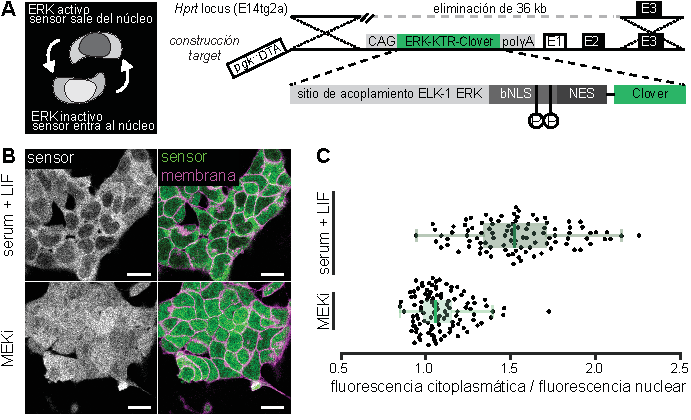
\includegraphics[width=1\columnwidth]{figures/chapter2/C2_KTR.pdf} 
    \caption{\textbf{Sensor de traslocación que permite medir la activación de ERK en mESCs vivas individuales.} (A) Principio de funcionamiento del sensor KTR (izquierda), y esquema del sensor KTR y su región de integración en el genoma (derecha). (B) Localización del sensor KTR en células vivas en s+L sin (arriba) y con MEKi (abajo). Las membranas están teñidas con el colorante de membrana de células vivas CellMaskRed. Barra de escala: 20 $\mu m$. (C) Cociente entre la fluorescencia citoplasmática y nuclear del sensor en células individuales obtenidas como en B. Las cajas verdes indican las medianas (mediana S+L = $1.52$, mediana MEKi = $1.05$; CV S+L = $0.18$, CV MEKi = $0.13$), los límites de la caja son los percentiles 25 y 75 de las distribuciones, y los bigotes son los percentiles 5 y 95. Los detalles del experimento se encuentran en \cite{Fabris2022}.}
    \label{C2_fig:KTR}
\end{figure}


En la figura \ref{C2_fig:KTR}B presentamos una foto de células con el sensor KTR integrado en mESCs. En el caso de las células que crecían en s+L, el sensor se localizó preferentemente en el citoplasma, aunque notamos cierta variabilidad en su localización preferencial. En contraste, en el control tratado con MEKi el sensor se distribuía uniformemente sobre toda la célula. Observamos en la figura \ref{C2_fig:KTR}C que este cociente era más variable entre las células que crecían en s+L que en el control tratado con MEKi, en consonancia con la marcación heterogénea de pERK de la figura \ref{C2_fig:inmuno}A. Estas similitudes cualitativas sugirieron que este sensor es adecuado para explorar la dinámica de ERK en mESCs.


En la figura \ref{C2_fig:KTR} comprobamos que la localización del sensor KTR correlacionaba con la activación de ERK. Sin embargo, nos quedaba determinar si este sensor era capaz de capturar la dinámica de esta activación. Para validar el sensor, cotransfectamos a las células con el KTR integrado con un sensor alternativo de la dinámica de activación de ERK y ortogonal al KTR. Este sensor era el ensamblado EKAREV-NLS, en donde EKAREV es un biosensor unimolecular FRET que mide actividad de ERK, cuyos donor y receptor eran los fluoróforos CFP (por \textit{cyan fluorescent protein}) e YFP (por \textit{yellow fluorescent protein}) respectivamente \cite{Komatsu2011} (sección \ref{C1_sec:ERK}). En este sensor, el sustrato que es fosforilado por pERK tiene una secuencia diferente al sustrato del KTR. Además, por EKAREV estar acoplado a una NLS, este sensor FRET monitorea la actividad de ERK en el núcleo de células vivas, donde mayores niveles de cociente FRET se corresponden con mayores niveles de actividad de ERK. Para que los espectros del sensor FRET y el KTR fueran compatibles, elegimos integrar a las células que cotransfectamos un sensor KTR que tenía acoplada otra proteína fluorescente (KTR-mCherry en lugar de KTR-mClover).


\begin{figure}
    \centering
    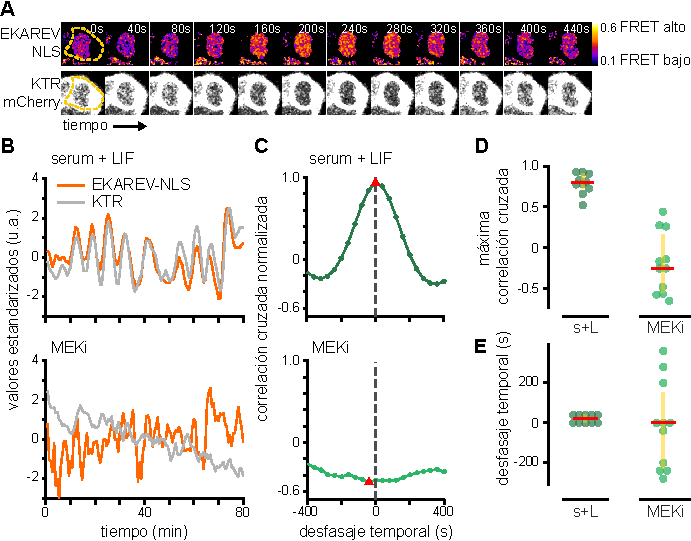
\includegraphics[width=1\columnwidth]{figures/chapter2/C2_FRET.pdf} 
    \caption{\textbf{Sensor FRET ortogonal al KTR reporta una dinámica similar.} (A) Cuadros de una mESCs (marcada en amarillo a los 0s) creciendo en s+L co-transfectada con los sensores EKAREV-NLS (arriba) y KTR-mCherry (abajo). En el fotomontaje del sensor EKAREV-NLS, se reporta el cociente entre la adquisición en el canal del aceptor y el donante, una vez estimulado el donante. En el del KTR, suavizamos la imagen con el único propósito de visualizarla y el valor de gamma se ajustó a $0.86$. La frecuencia de adquisición fue de $40$ s/cuadro. (B) Intensidad nuclear media de la imagen invertida (sensor KTR, gris) y el cociente FRETmedio (sensor EKAREV-NLS, naranja) en la misma región de interés nuclear a lo largo del tiempo en ausencia (arriba) y en presencia de MEKi (abajo). Las series temporales fueron estandarizadas, donde substrajimos la media y dividimos por la desviación estándar de cada serie temporal individual. (C) Correlación cruzada normalizada para los datos mostrados en B entre las series temporales de los diferentes sensores en función del tiempo de retardo. Su valor absoluto máximo está indicado (triángulo rojo). (D) Resumen estadístico de los valores absolutos máximos de las correlaciones cruzadas normalizadas entre ambos reporteros a lo largo de un desfase de $\pm$ $400 s$. (E) Resumen estadístico del desfasaje temporal en la máxima correlación cruzada normalizada. (D,E) La barra roja indica la mediana, la barra vertical amarilla indica la región entre el percentil 25 y el 75 de la distribución. Número de células: $n = 10$ (s+L), y $n = 11$ (MEKi). (A-E) Los detalles del experimento se encuentran en \cite{Fabris2022}.}
    \label{C2_fig:FRET}
\end{figure}

Observamos que la alta actividad de ERK detectada por el sensor FRET coincidía con una fuerte exclusión nuclear del reportero KTR (cuadro de 200 s. en figura \ref{C2_fig:FRET}A). Además, las cuantificaciones de ambos sensores mostraban un comportamiento dinámico similar (figura \ref{C2_fig:FRET}B). Para cuantificar esta comparación, calculamos la correlación entre las series temporales obtenidas para una misma célula por cada uno de los sensores (figura \ref{C2_fig:FRET}C-E). Observamos que los sensores estaban altamente correlacionados. Al los sensores KTR y EKAREV-NLS que utilizamos tener sitios \textit{target} de fosforilación diferentes, reportan la actividad de ERK de manera complementaria. Luego, la alta correlación que observamos entre estos dos sensores nos sugiere que el sensor de traslocación KTR es válido para reportar la actividad genuina de ERK a lo largo del tiempo.  


\subsection{Mediciones revelan actividad pulsátil de ERK}
\label{C2_ssec:tracking}

Una vez validado el sensor, el siguiente paso consistió sistematizar la adquisición de datos en una población representativa de células crecidas en s+L con y sin MEKi, y cuantificar estas mediciones. Primero filmamos células con el sensor KTR integrado con una resolución de $20$ segundos por cuadro y durante un máximo de $2$ horas. En las filmaciones, observamos una translocación repetitiva del sensor entre el citoplasma y el núcleo en el caso de células en s+L, efecto que no observamos en la condición con MEKi (figura \ref{C2_fig:citoplasma_nucleo}A  ,\href{http://movie.biologists.com/video/10.1242/dev.199710/video-1}{película ESCs}). 


Para cuantificar la información presente en las películas, en otras líneas celulares se había utilizado el cociente entre la intensidad media del citoplasma y del núcleo (C/N) como lectura de la actividad de ERK \cite{Regot2014}. Por tanto, era necesario realizar un \textit{tracking} del citoplasma y el núcleo de las células. El núcleo era fácil de detectar con nuestra vista, pero el citoplasma de cada célula era estrecho y difícil de distinguir (figura \ref{C2_fig:citoplasma_nucleo}A, \href{http://movie.biologists.com/video/10.1242/dev.199710/video-1}{película ESCs}). Por esto, y por el hecho de que las células se movían en las tres dimensiones del espacio, los algoritmos de segmentación con los que se suele automatizar este tipo de mediciones no funcionaban y decidimos realizar el seguimiento en forma semi-manual. En el \textit{tracking} semi-manual dibujamos manualmente regiones de interés (ROIs, por \textit{regions of interest}) cada 5 cuadros. Para la ROI nuclear, intentamos capturar toda el área nuclear, y en el caso del citoplasma seleccionamos regiones contiguas que pudieran ser asignadas inequívocamente a una célula específica. A continuación, utilizamos la función de interpolación de FIJI para tomar medidas en cada cuadro. De esta manera, realizamos el resto del \textit{tracking} de forma automática utilizando el \textit{plugin} \textit{Trackmate} para FIJI/ImageJ \cite{Tinevez2017}, inicialmente para toda la colonia. Luego, lo corregimos manualmente cuadro a cuadro. En este proceso descartamos las células que no mostraban un citoplasma pequeño y núcleo redondo bien definidos, morfología típica de las ESCs, y las células que salían del campo de visión. Las mediciones comenzaron al principio de la película, y se extendieron hasta su final o hasta una división celular. 


Adquirimos la intensidad media de fluorescencia en las ROIs de tamaño variable en ambos compartimentos. En la figura \ref{C2_fig:citoplasma_nucleo}B mostramos que caídas en la fluorescencia media del núcleo se condecían con aumentos en la fluorescencia media citoplasmática. Es decir, una reducción de la concentración del sensor KTR en el núcleo correlacionaba con un aumento de la misma en el citoplasma, y ambas eran mediciones complementarias del perfil de activación de ERK. Con esta información, sumado a que el \textit{tracking} semi-manual que implementamos era muy ineficiente para seguir el citoplasma celular, nos preguntamos si podíamos construir otro observable que mejore la eficiencia de esta cuantificación.


Comparamos la relación C/N con la señal nuclear adquirida como la intensidad media de una región de interés nuclear. Para la medición en el núcleo, invertimos los valores de fluorescencia. De esta manera, los valores de baja intensidad correspondan a una baja actividad de ERK, y los valores de alta intensidad indican una alta actividad de ERK (figura \ref{C2_fig:citoplasma_nucleo} B). Encontramos que estas dos señales eran muy similares y, por conveniencia, sistematizamos las mediciones de la localización del sensor en función del tiempo adquiriendo la intensidad media de una ROI nuclear sobre la imagen invertida, que en adelante llamaremos señal de KTR. De esta manera, los valores altos de la señal de KTR reflejaban una alta actividad de ERK.


\begin{figure}
    \centering
    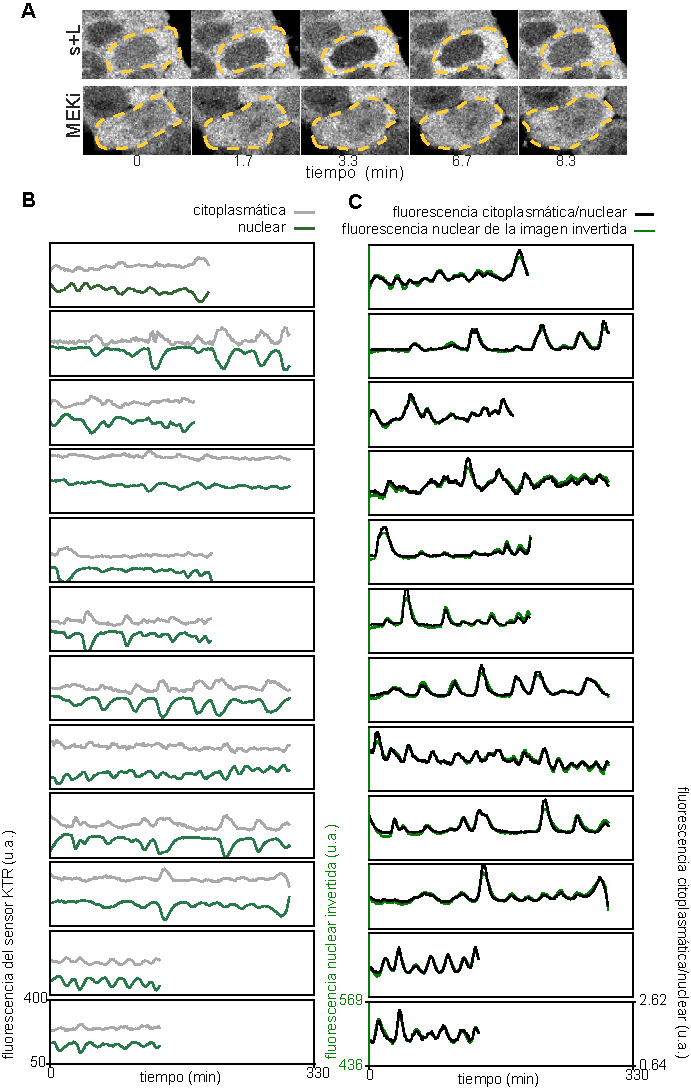
\includegraphics[width=1\columnwidth,scale =0.95]{figures/chapter2/C2_citoplasma_nucleo.pdf} 
    \caption{\textbf{La fluorescencia del sensor KTR medida en una región de interés nuclear capta la misma dinámica que la relación fluorescencia citoplasmática / nuclear.}(A) Cuadros de una película de células que expresan el sensor KTR de ERK, integrado a células creciendo en s+L sin (arriba) y con MEKi (abajo). La línea amarilla discontinua indica el contorno de una célula. (B) Fluorescencia media de del sensor KTR en regiones de interés citoplasmáticas (gris) y nucleares (verde). Cada cuadro representa la medición en una célula distinta. (C) Relación de la fluorescencia citoplasmática y nuclear de A (negro), y la intensidad media de la ROI nuclear medida en la imagen invertida (verde). En todos los casos, los ejes y se centraron en la media y se escalaron para abarcar 10 desviaciones estándar.}
    \label{C2_fig:citoplasma_nucleo}
\end{figure}


En la figura \ref{C2_fig:traces} presentamos la intensidad media de una región de interés nuclear para una población de células. Esta cuantificación reveló una amplia gama de comportamientos dinámicos en toda la población: algunas células mostraron actividad pulsátil regular (por ej., las células $0$ ó $40$), y otras mostraron solamente pulsos aislados (por ej., célula $14$). También observamos transiciones entre el comportamiento de pulsado y no pulsado dentro de la misma célula (por ej., células $33$ ó $52$), y de pulsos aislados (por ej., célula $42$). En resumen, encontramos que que las ESCs pluripotentes cultivadas en s+L mostraban una amplia gama de dinámicas de actividad pulsátil de ERK, ausente en la condición control.


%Como continuación, buscamos construir una descripción cuantitativa de la dinámica de activación de ERK, enfocándonos en describir este abanico de comportamientos dinámicos que identificamos cualitativamente. 


\begin{figure}
    \centering
    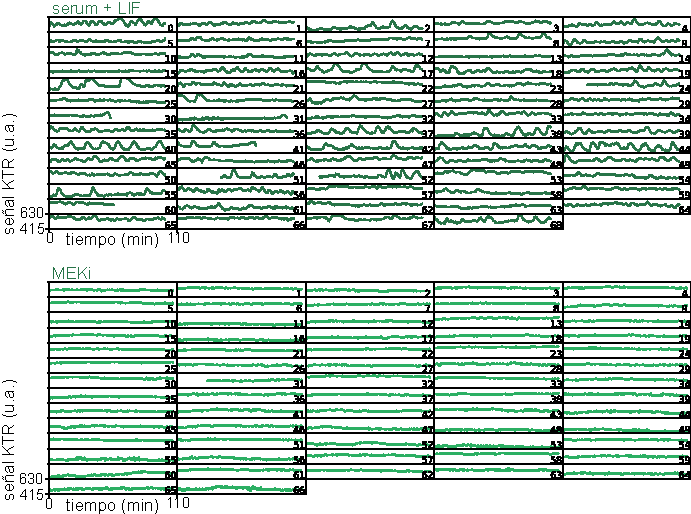
\includegraphics[width=1\columnwidth]{figures/chapter2/C2_traces.pdf} 
    \caption{\textbf{La dinámica de la señal KTR revela que la actividad de ERK es pulsátil en células madre embrionarias.} Series temporales de células individuales de la señal KTR, obtenidos como la intensidad media de una ROI nuclear medido en la imagen invertida, para células que crecen en s+L sin (arriba) y con MEKi (abajo). La disminución de la señal KTR al final de las series temporales en las células 30, 31, 41 y 50 en la condición sin MEKi se debe a la ruptura de la envoltura nuclear cuando las células entran en mitosis. Esta parte de la medición, junto con el pico inmediatamente anterior, se recortó para el análisis posterior. La tasa de adquisición fue de $20$ s/cuadro.}
    \label{C2_fig:traces}
\end{figure}




\section{Signos de oscilaciones en la actividad dinámica de ERK}
\label{C2_sec:oscilaciones}

Nuestras mediciones de la dinámica de activación de ERK en escalas temporales cortas revelaron una actividad pulsátil, donde algunas series temporales mostraban intervalos de actividad pulsátil regular donde los pulsos ocurrían uno a continuación del otro. A partir de esta observación surge naturalmente la pregunta de si estos intervalos son oscilatorios. Con esta motivación, en esta sección primero estudiamos los signos oscilatorios globales de las series temporales experimentales individuales a partir de analizar su espectro de potencias y su función de autocorrelación. Luego, utilizamos la transformada \textit{Wavelet} para estudiar su espectro local y determinar si existen signos oscilatorios no estacionarios. 


\subsection{El espectro de potencias y la función de autocorrelación recapitulan signos oscilatorios}
\subsectionmark{El espectro de potencias y la función de autocorrelación ...}


Para evaluar la hipótesis de que los intervalos de actividad pulsátil regular donde los pulsos ocurrían uno a continuación del otro se trataban de intervalos oscilatorios implementamos herramientas de análisis de oscilaciones estándares como son la Transformada de Fourier y la Función de Autocorrelación. Si bien el espectro de Fourier y de Autocorrelación están conectados por el Teorema de Wiener-Khinchin para series temporales infinitas \cite{Gardiner}, en nuestras mediciones las series temporales tienen una duración finita y un número pequeño de ciclos, y decidimos implementar ambos métodos de análisis. 


Previo a implementar estas herramientas, establecimos en cero la linea de base de las series temporales de la figura \ref{C2_fig:traces}. Es decir, para cada valor de la señal de KTR $x_i$, calculamos un nuevo valor $y_i$ como
\begin{equation}
    y_i = x_i - \frac{\sum_{j=0}^{n-1} x_j}{n},
    \label{C2_eq:base_cero}
\end{equation}
donde $0 \geq i > n-1$ denota el número de cuadro en el que fue adquirido $x_i$ dentro de la $n$ la cantidad de cuadros de cada serie temporal. Con esta definición, la nueva serie temporal resultante $y_i$ con $0 \geq i > n-1$ tiene un valor medio temporal nulo.


Para analizar el espectro de potencias de las series temporales, utilizamos la transformada discreta de Fourier.\marginpar{transformada de\\Fourier} Con esta operación es posible obtener una representación en frecuencias de una secuencia discreta y de duración finita que originalmente depende del tiempo, como es el caso de las series temporales de actividad de ERK que adquirimos experimentalmente. La idea detrás de esta estrategia es que la representación en frecuencias de un sistema dinámico oscilatorio tendrá picos o máximos en las frecuencias a las que oscila. Para implementar la transformada discreta de Fourier utilizamos el algoritmo de transformada rápida de Fourier. En nuestra implementación, elegimos descomponer las series temporales en una base de Fourier ortonormal que cumple la identidad de Parseval. Definimos, entonces, el espectro de amplitud de Fourier $A_k$ como \cite{Harris2020}
\begin{equation}
   A_k = \frac{1}{\sqrt{n}} \sum_{m=0}^{n-1} y_m \exp{(-2\pi i \frac{mk}{n})} \quad 0 \leq k \leq n-1,
   \label{C2_eq:amplitud_fourier}
\end{equation}
donde $n$ es el número de puntos de la serie temporal, y la base de frecuencias angulares asociadas es $\omega_k = 2\pi k/n$ con $0 \leq k \leq n-1$. En la figura \ref{C2_fig:FFT_AC}A observamos el espectro de potencias $|A_k|^2$ asociado a las frecuencias positivas de cada serie temporal de la figura \ref{C2_fig:traces}. 


 \begin{figure}
    \centering
    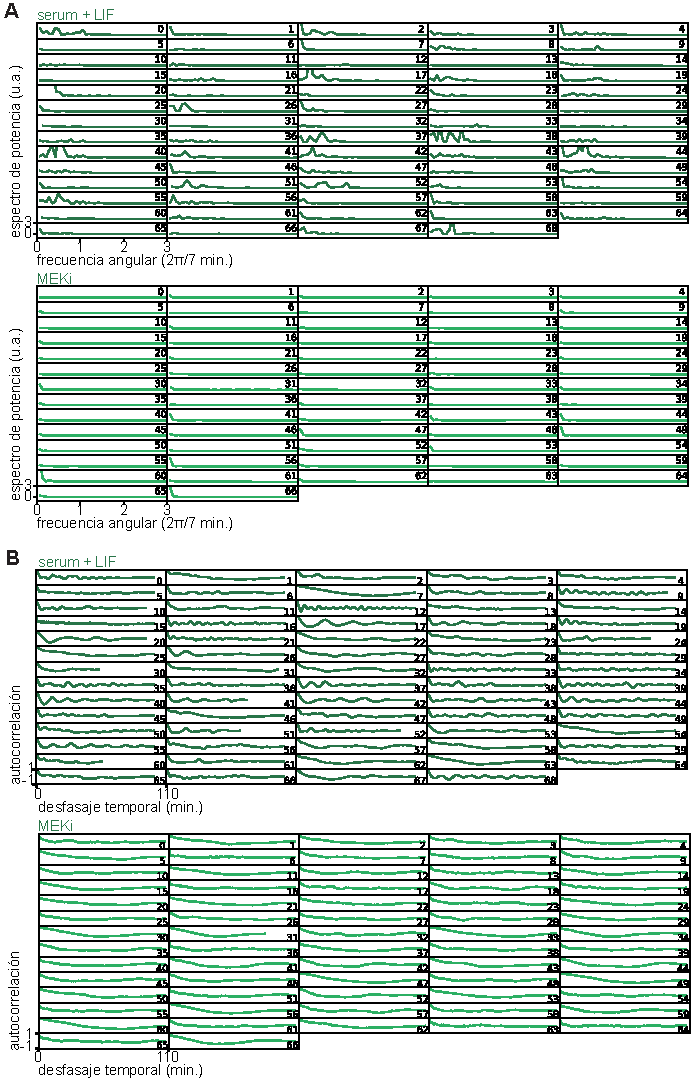
\includegraphics[width=1\columnwidth]{figures/chapter2/C2_FFT_AC.pdf}
    \caption{\textbf{Signos oscilatorios globales en mESCs que crecen en s+L.} (A) Espectro de potencia y (B) función de autocorrelación de las series temporales de actividad de ERK adquiridas en células individuales de la figura \ref{C2_fig:traces}. En A la escala del eje x es $ 2\pi/7\; \text{min}^{-1}$.}
    \label{C2_fig:FFT_AC}
\end{figure}


Para la condición control de ESCs \textit{wild type} individuales crecidas en s+L y Meki, observamos un espectro de potencias mayoritariamente plano y sin un valor preferencial. En algunos casos, como por ejemplo las células $60$ ó $66$, notamos un pico en el rango de las frecuencias bajas. Este pico sugiere que para algunos casos existe una tendencia global o \textit{trend} en las series temporales. En cambio, en el caso de ESCs \textit{wild type} individuales crecidas en s+L, el espectro de potencias sugiere un comportamiento oscilatorio en un subconjunto de series temporales, en contraposición con la condición control. Observamos un rango preferencial de frecuencias en el espectro de potencias, por lo general en escalas temporales menores a $7$ minutos, en casos en donde observábamos comportamientos puramente pulsátiles como por ejemplo las células $40$ ó $44$ de la figura \ref{C2_fig:traces}. Por otro lado, el análisis mostró que en algunas otras series temporales no había rango preferencial de frecuencias, por ejemplo las células $15$ ó $31$. Esta información se condice con la inspección visual de estas series temporales en la figura \ref{C2_fig:traces}. Otro conjuntos de células, por ejemplo la $4$ o la $7$, presentaban dentro de su espectro ciertas frecuencias preferenciales muy pequeñas, efecto similar al observado para la condición control. En varios ejemplos, aparte de esa frecuencia baja, se podía distinguir otro rango de frecuencias sugerente de oscilaciones (comparar célula $4$ con célula $7$). Además, en ciertos casos, por ejemplo las células $52$ ó $55$, aparecían por lo menos dos picos en el espectro de potencias. Interpretamos que este efecto es consecuencia de cuando hay pulsos o intervalos pulsátiles intercalados con intervalos de no pulsado. 


Como complemento, la función de autocorrelación consiste en la convolución de una señal consigo misma. Es una medida de similaridad entre sí misma y su versión retardada, y es útil para encontrar patrones repetitivos en señales con ruido. La autocorrelación de una señal oscilatoria tendrá ciclos con la escala temporal de las oscilaciones. A continuación, calculamos la función de autocorrelación como \cite{Harris2020} \marginpar{función de\\autocorrelación}
\begin{equation}
    [y \cdot y]_\tau = \frac{1}{N} \sum_{m = -\infty}^{\infty} y_m \; y^*_{\tau - m},
\end{equation}
donde $y^*_m$ es el complejo conjugado de $y_m$, $\tau$ es un desfasaje temporal, y $N = \sum_{m = - \infty}^{\infty} y_m^2$ la constante de normalización. Los límites del índice temporal $m$ los representamos como infinito, pues rellenamos la serie temporal $x_m$ con ceros cuando fue necesario. En la figura \ref{C2_fig:FFT_AC}B presentamos el análisis de autocorrelación para las series temporales de la figura \ref{C2_fig:traces}. Para el caso del control con MEKi, observamos que la autocorrelación de las series temporales muestran ciclos de baja amplitud y escalas temporales largas, posiblemente debido a tendencias globales o \textit{trends}. Al igual que el análisis de Fourier, la autocorrelación de las trazas individuales en s+L mostró signos de oscilaciones, aunque muy variables, en un subconjunto de células. Si nos enfocamos en las células $40$ o $44$, podemos ver ciclos de amplitud variable que decaen gradualmente con el tiempo, característica de dinámicas oscilatorias en donde hay variabilidad en el tiempo entre picos. En algunos casos, por ejemplo las células $12$ ó $16$, la autocorrelación parecía evidenciar patrones oscilatorios más claramente que el análisis de Fourier. Por otro lado, las series temporales que no pulsan tienen una función de autocorrelación plana o decaimientos muy suaves. Si bien este análisis resultó más conveniente para distinguir comportamientos puramente oscilatorios, las células con pulsos  o intervalos pulsátiles intercalados con intervalos de no pulsado, por ejemplo la $52$, eran difíciles de interpretar.



Recapitulando, estas herramientas de análisis de oscilaciones sugieren un comportamiento oscilatorio en una porción de los datos de s+L, y la heterogeneidad de los resultados respalda la idea de que la actividad de ERK viene en un abanico de comportamientos dinámicos distintos. Sin embargo, resultaron insuficientes para caracterizar los diferentes rasgos dinámicos que observábamos, por ejemplo, los trenes de pulsos entre intervalos de no pulsado. Con estas ideas, proponemos utilizar herramientas alternativas para intentar distinguir los signos oscilatorios locales de las series de actividad dinámica de ERK. 



\subsection{El espectro \textit{Wavelet} sugiere que las oscilaciones son no estacionarias}

La transformada \textit{Wavelet} es una herramienta popular para analizar series temporales cuyo espectro de potencias no es estacionario, dado que extrae simultáneamente información local espectral y temporal. \marginpar{transformada Wavelet} Se trata de la convolución local entre la serie temporal discreta $y_i$ con una función \textit{wavelet madre} $\Psi(\eta)$ \cite{Torrence1998}. Se acostumbra que la wavelet madre parezca una oscilación breve, y la forma de sus pulsos suele elegirse para que sean similares a la forma de los pulsos de las series temporales que se busca analizar. En resumen, la amplitud del espectro de Wavelet $W_k(s)$ se calcula como
\begin{equation}
    W_k(s) = \sum_{m=0}^{n-1} y_m \Psi^* \Big[ \frac{(m-k) \delta t}{s}\Big], 
 \end{equation}
donde $s$ es la escala de la Wavelet, $n$ la cantidad de puntos de la serie temporal, $\delta t$ su resolución temporal,  y $*$ indica complejo conjugado. Aquí empleamos como función \textit{wavelet madre} $\Psi(\eta)$ a la función de Morlet, una onda plana modulada con una gaussiana
\begin{equation}
 \Psi(\eta) = \pi^{-1/4} \; e^{i\omega_0 \eta } e^{-\eta^2 / 2}.
\end{equation}
Esta función tiene un solo parámetro, la frecuencia adimensional $\omega_0$ que fijamos en $6$. Con esta elección de parámetros, la envolvente gaussiana decae de manera que la Wavelet madre tiene aproximadamente tres ciclos. 


Como estamos trabajando con series temporales finitas, rellenamos las series temporales con ceros cuando fue necesario. Sin embargo, existen efectos de borde al principio y al final de cada espectro. El cono de influencia es la región del espectro Wavelet en la que los efectos de borde comienzan a ser importantes. En este trabajo la definimos como el tiempo en que la autocorrelación de la Wavelet decae un factor $1/e^2$ \cite{Torrence1998}. 

 \begin{figure}
    \centering
    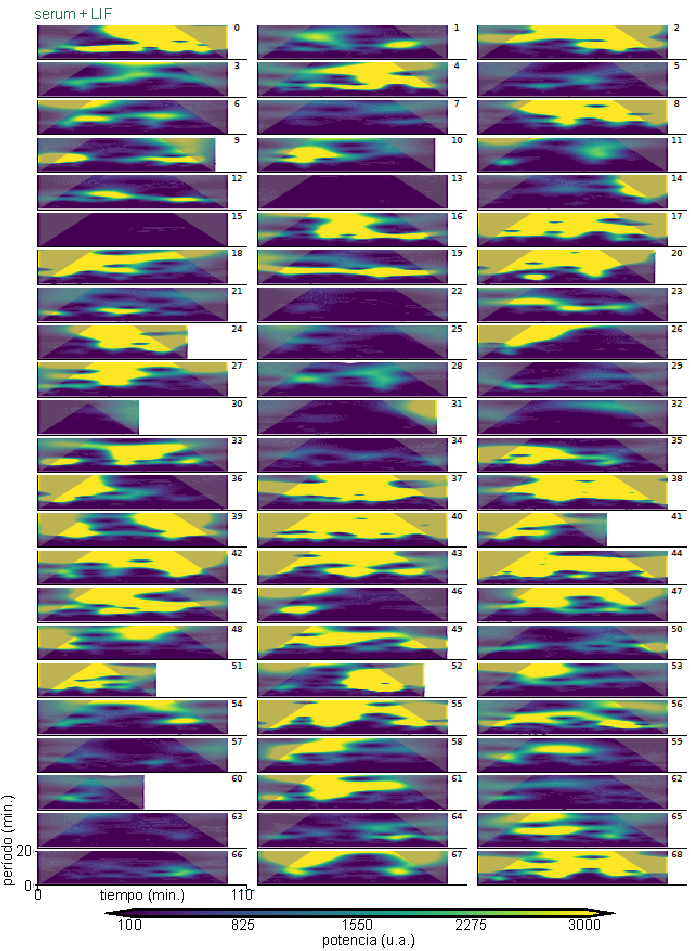
\includegraphics[width=1\columnwidth]{figures/chapter2/C2_wavelets_WT.pdf}\caption{\textbf{Signos de oscilaciones locales en la dinámica de activación de ERK.} Espectro de Wavelets de células individuales a partir de los datos de células que crecen en s+L de la figura \ref{C2_fig:traces}. La región gris marca el cono de influencia.}
    \label{C2_fig:wavelets_WT}
\end{figure}


 \begin{figure}
    \centering
    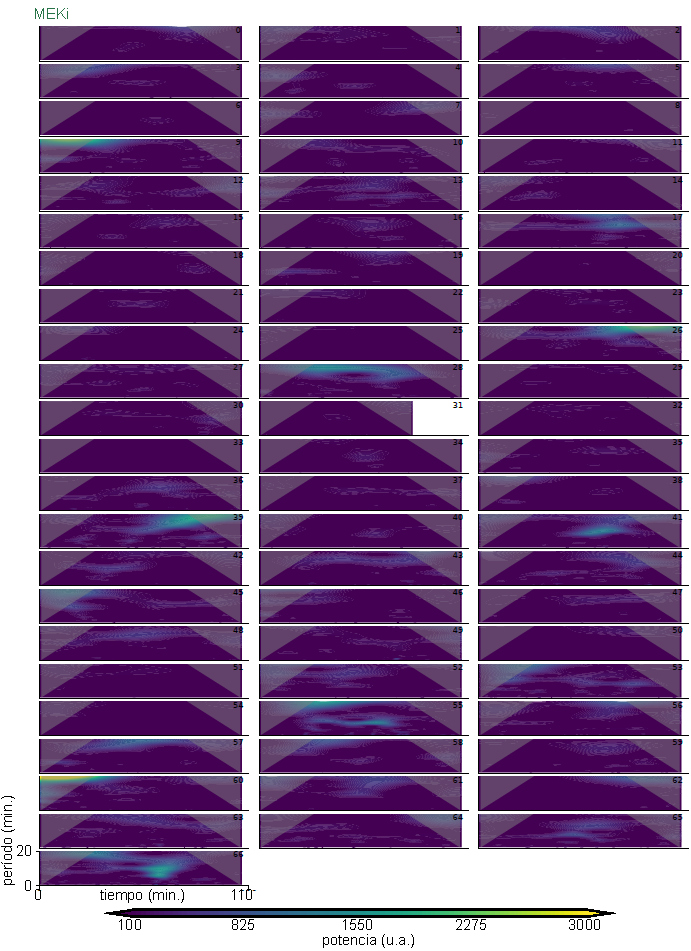
\includegraphics[width=1\textwidth]{figures/chapter2/C2_wavelets_MEKi.pdf}\caption{\textbf{Signos de oscilaciones locales en la dinámica de activación de ERK.} Espectro de Wavelets de células individuales a partir de los datos de células que crecen con MEki de la figura \ref{C2_fig:traces}. La región gris marca el cono de influencia.}
    \label{C2_fig:wavelets_MEKI}
\end{figure}


En la figura \ref{C2_fig:wavelets_WT} presentamos el espectro de Wavelet para las células que crecen en s+L, y en la figura \ref{C2_fig:wavelets_MEKI} para las células que crecen en s+L pero con MEKi. En ambos casos establecimos en cero la línea de base de las series temporales antes de implementar la transformada (ecuación \ref{C2_eq:base_cero}). Presentamos los resultados de este análisis en un gráfico donde el eje $x$ corresponde a escala temporal de las series temporales, y el eje $y$ es el período del espectro Wavelet. La escala de color representa la potencia del espectro Wavelet. Si, por ejemplo, analizáramos una función sinusoidal de período $T$, veríamos una recta horizontal en $y = T$. Si esa oscilación ocurre sólo entre los tiempos $t_1$ y $t_2$, esta recta estaría acotada en el eje $y$ en ese mismo intervalo.   


Comparando las figuras \ref{C2_fig:wavelets_MEKI} con \ref{C2_fig:wavelets_WT}, es notoria la presencia de actividad en el caso de las células crecidas en s+L. En algunos casos detectamos la presencia de oscilaciones a lo largo de casi toda la serie temporal, por ejemplo en las células $0,\; 19$ ó $37$. El período de estas oscilaciones estaba alrededor de los $10$ minutos, aunque las franjas que indican la presencia de oscilaciones eran anchas y poco precisas. Muchas veces se recurre a estrategias de filtrado para evitar estos efectos, a costa de la posibilidad de introducir sesgos espectrales, como por ejemplo la atenuación o amplificación de ciertas frecuencias \cite{Monke2020}. Por esta razón en este trabajo decidimos realizar un análisis cualitativo y evitar filtrar las series temporales. 

Respecto a rasgos oscilatorios locales, observamos altos valores de frecuencias localizados en células como por ejemplo la $39$ o la $52$, sugiriendo intervalos oscilatorios acotados en las series temporales. Sin embargo, los pulsos aislados se confundían con oscilaciones locales (por ejemplo, la célula $42$), o no eran correctamente detectados (por ejemplo, la célula $28$). 
 
En la figura \ref{C2_fig:wavelets_MEKI} podemos observar que no hay signos oscilatorios, y la mayoría de las células muestran una potencia baja y uniforme. En algunos casos, por ejemplo en las células $26$ ó $28$, se observan pequeñas variaciones de períodos largos. En células como la $55$ o la $66$, se observan pequeños incrementos en la potencia a períodos cortos. Cuando observamos las correspondientes series temporales en la figura \ref{C2_fig:traces}, vemos que estos pequeños incrementos probablemente se deban a fluctuaciones producto del ruido y no reflejan ningún comportamiento dinámico. 


En definitiva, este análisis espectral nos reafirma que las oscilaciones de actividad de ERK no son estacionarias, y los intervalos oscilatorios tienen una escala temporal de alrededor de $10$ minutos. No obstante, para construir una descripción conceptual de la dinámica de ERK, consideramos importante incorporar la presencia de intervalos oscilatorios y simultáneamente pulsos aislados. Con este análisis, esto no parece ser posible, y decidimos proponer una nueva herramienta de análisis para caracterizar la dinámica de activación de ERK que incorpore estos elementos. 


\section{Detección de pulsos de actividad}
\label{C2_sec:pulse_detection}

En la sección \ref{C2_sec:mediciones} observamos en las series temporales que representan la actividad dinámica de ERK que algunas células presentaban intervalos de actividad pulsátil regular, que en la sección \ref{C2_sec:oscilaciones} describimos como oscilaciones no estacionarias. El comportamiento oscilatorio coexiste con pulsos aislados e intervalos donde no hay actividad pulsátil. Este abanico de comportamientos nos sugiere que los bloques elementales de la dinámica son los pulsos. 

Para construir una caracterización cuantitativa de la dinámica de activación de ERK, nos preguntamos cómo son las propiedades dinámicas de sus bloques elementales, los pulsos, y cómo éstos se organizan en las series temporales. En esta sección desarrollamos un protocolo de detección de pulsos que nos permitirá estudiar las características dinámicas de las series temporales que representan la dinámica de activación de ERK de manera sistemática y cuantitativa. Este protocolo comienza con un preprocesamiento que busca aumentar la calidad de información sobre la dinámica de activación de ERK en las series temporales. Luego, presentamos el algoritmo de detección de pulsos, que es general para series temporales de características similares a las que adquirimos en los experimentos, y finalmente presentamos el método de calibración del algoritmo, donde buscamos detectar pulsos de actividad en las series temporales de activación de ERK experimentales. 


\subsection{Preprocesamiento de la señal}


Examinamos las series temporales con el fin de detectar, y posteriormente corregir o evitar, errores de \textit{tracking}. Por ejemplo, cuando las ROIs se situaban por error parcialmente fuera del núcleo en el citoplasma, o que se solapaban con un nucleolo. Como tanto el citoplasma como los nucleolos tenían intensidades de fluorescencia que normalmente diferían de las del nucleoplasma (\href{http://movie.biologists.com/video/10.1242/dev.199710/video-1}{película ESCs}), estos errores normalmente conducían a un aumento en la varianza de la intensidad de los píxeles que componían la ROI. Examinamos las series temporales en busca de regiones de alta varianza, considerando como alta varianza a las que superaban el valor de umbral establecido manualmente y que era propio de cada conjunto de datos. Una vez identificadas estas regiones, revisamos el \textit{tracking} y lo corregimos si era necesario.


Por otro lado, justo antes de la división celular, el sensor KTR se excluía del núcleo (\href{http://movie.biologists.com/video/10.1242/dev.199710/video-1}{película ESCs}). Este efecto daba lugar a un pulso de alta amplitud al final de las series temporales correspondientes a células que se dividían (por ejemplo, las células $30,\; 31,\; 41$ y $50$ en la condición s+L sin MEKi, figura \ref{C2_fig:traces}). Este efecto fue observado tanto en la condición de s+L, como en la condición con el inhibidor MEKi. Esto sugiere que este pulso no es informativo de la actividad de ERK. Decidimos recortar estos eventos, y eliminamos los últimos $20$ cuadros (unos $7$ minutos) de las series temporales asociadas a células que se dividían. 


\subsection{Algoritmo de detección}
\label{C2_ssec:algoritmo}

Una vez conformes con la calidad de información sobre la dinámica de activación de ERK en las series temporales, buscamos detectar pulsos de actividad en ellas, distinguiéndolos de sus fluctuaciones de base.\marginpar{pulso de actividad} Para esto, definimos un \textbf{pulso de actividad} como un máximo local entre dos mínimos locales, imponiendo dos condiciones: (i) requerimos que la amplitud del pulso sea mayor que un umbral de amplitud $A_{\text{th}}$, y que, (ii) en promedio, las pendientes del pulso sean mayor que un umbral de pendiente $v_{\text{th}}$. Estos dos umbrales son parámetros libres del algoritmo, que establecimos a través de un protocolo de análisis cuantitativo de umbrales que desarrollamos para calibrar el algoritmo y describiremos más adelante (cuadro \ref{C2_tab:th_WT}). 


Las series temporales tenían ruido de alta frecuencia que interfería con el rendimiento del algoritmo de detección de pulsos. Por esta razón suavizamos las series temporales filtrando las frecuencias más altas. Para esto, utilizamos una ventana de media móvil de $3$ cuadros de duración. Para cada valor $x_i$ de la señal KTR de la serie temporal, calculamos el valor medio 
\begin{equation}
    \hat{x}_i = \frac{1}{3} ( x_{i-1} + x_{i} + x_{i+1} ) ,
\end{equation}
donde $i$ es el número de cuadro. En los bordes de las series temporales consideramos ventanas de $2$ y $1$ cuadro (figura \ref{C2_fig:algoritmo_pulse_detection}). Por el contrario, no fue necesario eliminar bajas frecuencias. 


Luego, buscamos en la serie temporal todos los máximos y mínimos locales. Para esto, comparamos cada valor $\hat{x}_i$ de la serie temporal con sus vecinos inmediatos $ \hat{x}_{i-1}$ y $ \hat{x}_{i+1}$. El valor inicial $\hat{x}_0$ se comparó solo con el siguiente valor $\hat{x}_1$, y el último valor $\hat{x}_{n-1}$ con el anterior $ \hat{x}_{n-2}$. Descartamos el primer máximo si no había ningún mínimo a su izquierda, y el último máximo si no había ningún mínimo a su derecha. De esta forma definimos un subconjunto de puntos $ M = \lbrace j | \hat{x}_j > \hat{x}_{j \pm 1}\rbrace$ formado por los máximos locales, y el subconjunto de mínimos locales $ m = \lbrace j | \hat{x}_j < \hat{x}_{j \pm 1}\rbrace$ (figura \ref{C2_fig:algoritmo_pulse_detection}). De la definición se deduce que la distancia mínima $|i-j|$ entre dos máximos $\hat{x}_i, \hat{x}_j \in M$ es de $2$ cuadros, y la distancia mínima $|k-l|$ entre dos mínimos $\hat{x}_k, \hat{x}_l \in m$ es de $2$ cuadros. 


Para determinar cuáles de estos máximos y mínimos locales definían un pulso, implementamos dos filtros simultáneamente: uno en amplitud y otro en pendiente. Recorrimos cada máximo de la serie temporal, de izquierda a derecha. Para cada máximo de índice $j \in M$ de valor $\hat{x}_j$, buscamos el primer mínimo a su izquierda de índice $k \in m$ de valor $\hat{x}_k$ con $k < j$ tal que la amplitud izquierda resultante $A_j^{\text{left}} = \hat{x}_j-\hat{x}_k$ fuera mayor que el umbral de amplitud $A_j^{\text{left}} \geq A_{\text{th}}$, y la pendiente izquierda (o de subida del potencial pulso) fuera mayor que el umbral de pendiente $v_j^{\text{left}} \geq v_{\text{th}}$. La pendiente izquierda se definió como $v_j^{\text{left}} = A_j^{\text{left}}/ dt_j^{\text{left}}$, donde $dt_j^{\text{left}}=j-k$ es la duración del pulso izquierdo. De manera similar, buscamos el primer mínimo a la derecha que verificara $A_j^{\text{right}} \geq A_{\text{th}}$  y $v_j^{\text{right}} \geq v_{\text{th}}$, donde $v_j^{\text{right}}$ es la pendiente de bajada del potencial pulso de actividad  (figura \ref{C2_fig:algoritmo_pulse_detection}, cuadro \ref{C2_tab:th_WT}).


Conservamos grupos de $2$ mínimos locales y un máximo local que cumplían con los criterios de umbrales establecidos. Como nada impedía que estos grupos de $3$ puntos no se solapen entre sí, buscamos eliminar los candidatos a pulso que se solapaban: si el mínimo derecho del primer pulso ocurría más tarde que este nuevo mínimo izquierdo del segundo, descartamos el pulso que tenía la menor amplitud, definida como $ (A_i^{\text{left}} +  A_i^{\text{right}})/2$ (figura \ref{C2_fig:algoritmo_pulse_detection}).


\begin{figure}
    \centering
    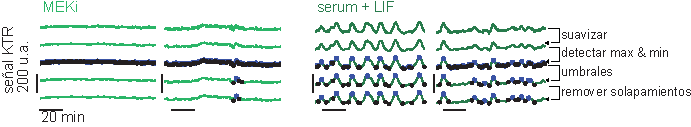
\includegraphics[width=1\columnwidth]{figures/chapter2/C2_algoritmo_pulse_detection.pdf} 
    \caption{\textbf{Algoritmo de detección de pulsos.} Series temporales representativas de la actividad dinámica de ERK en ESCs individuales que crecen en s+L en presencia (dos columnas a la izquierda) o ausencia (dos columnas a la derecha) de MEKi. Las filas ilustran los pasos del algoritmo de reconocimiento de pulsos: la primera fila muestra los datos crudos, la segunda fila muestra las series temporales suavizadas. Los puntos azules y negros de la tercera fila son máximos y mínimos locales. La cuarta fila muestra los máximos y mínimos locales que superan los umbrales de amplitud y pendiente. La quinta fila muestra los pulsos identificados tras eliminar los solapamientos. Los pulsos están definidos por los máximos y sus mínimos adyacentes.}
    \label{C2_fig:algoritmo_pulse_detection}
\end{figure}


\subsection{Determinación de umbrales}


El reconocimiento de los pulsos mediante la implementación del algoritmo desarrollado en \ref{C2_ssec:algoritmo} depende de los umbrales de amplitud $A_{\text{th}}$ y pendiente $v_{\text{th}}$. Para calibrar el método de detección para un dado conjunto de datos, es necesario determinar estos parámetros de manera sistemática en los datos correspondientes. Como en este trabajo el objetivo es detectar pulsos de actividad de ERK en las series temporales experimentales, proponemos calibrar el método de detección de pulsos a partir de dos ideas: (i) que las fluctuaciones de base dominan las series temporales del control negativo, condición en la que no se espera que ERK esté activo ; y (ii) que en la condición experimental donde ERK es más activo se busca que la detección de pulsos maximice la cantidad de pulsos detectados en esa condición. 


Para encontrar parámetros que garanticen estas dos condiciones, comenzamos por definir un espacio exploratorio bidimensional de parámetros $(A_{\text{th}}^m , v_{\text{th}}^n)$ (cuadro \ref{C2_tab:th_WT}). Luego, para cada combinación de parámetros $(A_{\text{th}}^m , v_{\text{th}}^n)$ en el espacio de parámetros exploratorio, implementamos el algoritmo de detección de pulsos descripto en el apartado \ref{C2_ssec:algoritmo} para el control negativo. A partir de su resultado calculamos la \textbf{tasa de pulsado promedio} como  \marginpar{tasa de pulsado promedio}
\begin{equation}
    \delta_\text{p} = \frac{1}{N} \sum_{j=1}^N \frac{n_j}{L_j},
\end{equation}
donde $N$ es el número total de células en el control negativo, $n_j$ es el número de pulsos detectados y $L_j$ es la duración de la serie temporal de la célula $j$ (figura \ref{C2_fig:umbrales}A). A partir de esta definición, si la tasa de pulsado promedio es alta, significa que hay muchos pulsos detectados y si es baja, que hay pocos. 


A continuación, restringimos el espacio exploratorio bidimensional a una curva de nivel exploratoria en el espacio de parámetros fijando los valores de la tasa de pulsado media $\delta_\text{p}= \delta_\text{p}^*$ en el control negativo (cuadro \ref{C2_tab:th_WT}, figura \ref{C2_fig:umbrales}A). Con esta definición, una curva de nivel exploratoria identifica pares de parámetros $(A_{\text{th}}^m , v_{\text{th}}^n)$  con la misma tasa de pulsado promedio. Elegimos valores de $\delta_\text{p}^*$ que se correspondían con un nivel bajo de pulsos detectados. En algunos casos, por inspección visual interpretábamos que había pulsos en el control negativo (por ejemplo, en la célula 55 de la condición con MEKi en la figura \ref{C2_fig:traces}), y con este criterio decidimos que el valor fijado no podía ser nulo para permitir la detección de esos pulsos. 


\begin{figure}
    \centering
    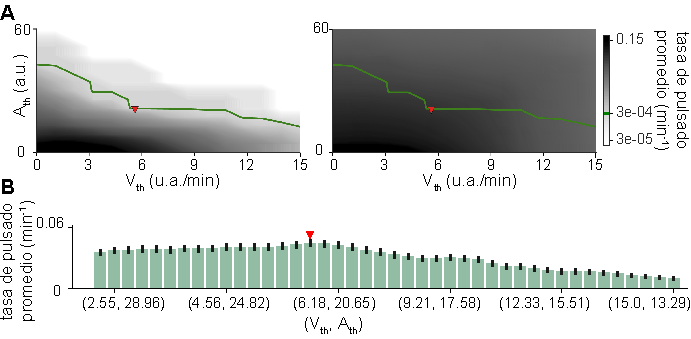
\includegraphics[width=1\columnwidth]{figures/chapter2/C2_umbrales.pdf} 
    \caption{\textbf{Análisis de umbrales para calibrar el algoritmo de detección de pulsos para las series temporales experimentales.} (A) Tasa media de pulsado en función de los umbrales de amplitud y pendiente para las células que crecen en s+L con (izquierda) o sin (derecha) MEKi. La curva de nivel en la que la tasa media de pulsado en las células tratadas con MEKi es de $3\times10^{-4} \text{min}^{-1}$ (línea verde) se utilizó para explorar combinaciones de valores de umbral de amplitud y pendiente en la condición sin inhibidor. (B) Tasa media de pulsado para combinaciones de umbrales de amplitud y pendiente a lo largo de la curva verde de A en células que crecen sólo en s+L. La barra de error indica la desviación estándar dividido la raíz cuadrada del tamaño de la muestra (SEM). El triángulo rojo en A,B indica los valores de los parámetros utilizados para el análisis posterior (cuadro \ref{C2_tab:th_WT}).}
    \label{C2_fig:umbrales}
\end{figure}


A continuación, para cada combinación $(A_{\text{th}}^{m_k} , v_{\text{th}}^{n_k})$ en cada curva de nivel exploratoria $k$, aplicamos el algoritmo de reconocimiento del pulsos en la condición experimental en la que la ERK era más activa, en este caso la condición con s+L. El gráfico de la tasa de pulsado a lo largo de esta curva de nivel mostró que la zona del espacio de parámetros donde la detección de pulsos era máxima era una región plana (figura \ref{C2_fig:umbrales}B). Dentro de esta región de tasa de pulsado similar, a partir de una inspección visual elegimos pares de parámetros que filtraran lo mejor posible los pulsos espurios, planos y largos del control negativo. Esto dio lugar a un par de parámetros $(A_{\text{th}}^m , v_{\text{th}}^n)$ específicos para cada experimento, que están detallados en el cuadro \ref{C2_tab:th_WT} y en la figura \ref{C2_fig:umbrales}B con un triángulo rojo.


Con esta calibración, la detección de pulsos dio como resultado que la mayoría de las células $(64/69, 93\%)$ presentaban pulsos de actividad en la condición de s+L, condición en la que se espera actividad de ERK, mientras que en la condición control una baja proporción de células que presentaban pulsos, $(2/67, 3\%)$.

\begin{table}[htbp]
\begin{adjustwidth}{-0.5in}{-0.5in}% adjust the L and R margins by 1 inch
\centering
\begin{tabular}{|l|l|l|l|l|l|l|}
\hline
 control & control & espacio & curva & umbral & umbral \\
 negativo & positivo & exploratorio & de nivel ($\delta_\text{p}^*$) & de & de \\
 &  & de parámetros & & amplitud & pendiente \\
\hline \hline
MEKi & serum + LIF & $v_{\text{th}}$ : (0,15) $\frac{\text{u.a.}}{\text{min}}$ & $3 \times 10^{-4} \frac{1}{\text{min}}$ & 20,68 u.a. & 5,61 $\frac{\text{u.a.}}{\text{min}}$ \\
 & & con res.: 0,25 $\frac{\text{u.a.}}{\text{min}}$ &  & & \\
 & & $A_{\text{th}}$ : (0,60) u.a. & & & \\
 & & con res.: 1 u.a. & & & \\
\hline
\end{tabular}
\end{adjustwidth}
\caption{Parámetros del algoritmo de detección de pulsos que surgieron del protocolo de análisis de umbrales para las series temporales de la figura \ref{C2_fig:traces}.}
\label{C2_tab:th_WT}
\end{table}


\section{Caracterización cuantitativa de la dinámica de pulsado}
\label{C2_sec:analisis}

En la sección \ref{C2_sec:pulse_detection} construimos un protocolo de detección de pulsos, elementos que consideramos como los bloques elementales de la actividad dinámica de ERK. El resultado de esta detección es un conjuntos de pulsos $P= \lbrace P_j=(j, kj, lj) | P_j \text{ es un pulso}$, donde cada pulso $P_i$ tiene asociados los índices $j$ (pico), $kj$ (inicio), y $lj$ (final). En esta sección presentamos la primera descripción cuantitativa de la dinámica de activación de ERK en células madre embrionarias en escalas temporales cortas, descripción que desarrollamos a partir de los resultados del algoritmo de detección. Explotando el hecho de que con el algoritmo de detección de pulsos fue posible identificar el inicio, el pico y el final de cada pulso, introducimos una serie de medidas cuantitativas. Estas medidas buscan estudiar, primero, las características dinámicas de pulsos individuales; luego, cómo es la actividad de ERK a lo largo de la población celular y; finalmente, cómo se organizan los pulsos en las series temporales experimentales.
 

\subsection{Amplitud y duración de pulsos individuales}

Para estudiar las características dinámicas de los pulsos de actividad individuales en la población celular, introdujimos un conjunto de medidas cuantitativas: la amplitud y la duración del pulso (figura \ref{C2_fig:amp_durac}A). 

 \begin{figure}
    \centering
    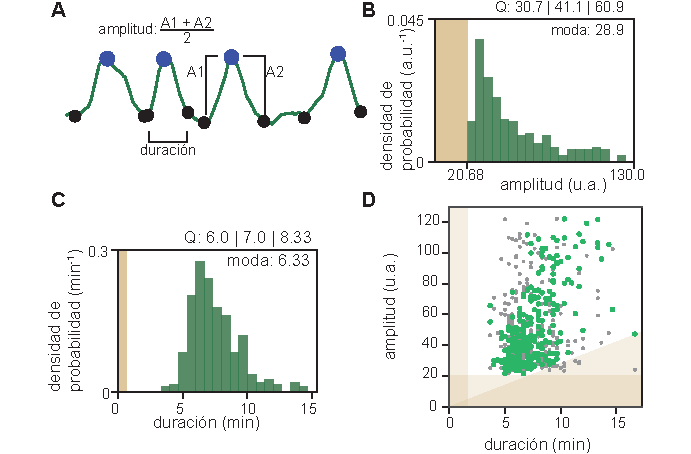
\includegraphics[width=1\columnwidth]{figures/chapter2/C2_amp_durac.pdf}\caption{\textbf{Caracterización cuantitativa de pulsos individuales.} (A) Amplitud y duración de pulsos indicadas en una porción de una serie temporal de célula individual suavizada de la señal KTR en la condición de s+L. Los pulsos se indican por los máximos (puntos azules) y los mínimos correspondientes (puntos negros) que los definen. (B) Distribución de la amplitud de los pulsos para la condición de serum + LIF. (C) Distribución de la duración del pulso para la condición de serum + LIF. (D) Amplitud de un pulso en función de su duración (puntos verdes). Los puntos grises muestran valores mezclados al azar para su comparación. El límite de resolución del reconocimiento de pulsos (barra amarilla) y los cuartiles (Q) 25, 50 y 75 se indican en (B,C). (B-D) N = 69 células, n = 289 pulsos.}
    \label{C2_fig:amp_durac}
\end{figure}

 Para cada pulso $P_i$ en el conjunto de pulsos $P= \lbrace P_j=(j, kj, lj) | P_j \text{ es un pulso} \rbrace$ definimos la \textbf{amplitud del pulso} $A_i$ como el promedio de sus amplitudes derecha e izquierda (figura \ref{C2_fig:amp_durac}A) \marginpar{amplitud}
\begin{equation}
    A_i = \frac{1}{2} (A_i^{\text{left}} +  A_i^{\text{right}}).
\end{equation}
Para la condición de s+L obtuvimos los resultados de la figura \ref{C2_fig:amp_durac}B, en donde en  amarillo se encuentra representado el valor umbral del algoritmo de detección de pulsos. Observamos que los umbrales que elegimos sólo filtran la cola de valores pequeños de la distribución de la amplitud de pulsos. Esta cola de bajas amplitudes contiene fluctuaciones que caen dentro del rango de los niveles de fluctuaciones determinados a partir de las series temporales de las células tratadas con MEKi. Luego, aunque no conocemos la relación funcional entre la actividad de ERK y la amplitud del pulso, a partir de esta distribución podemos confiar que nuestra tarea de distinguir pulsos de fluctuaciones estadísticas fue exitosa.


Continuamos definiendo la \textbf{duración de un pulso} $dt_i$ como la distancia entre los dos mínimos que lo definen (figura \ref{C2_fig:amp_durac}A) \marginpar{duración}
\begin{equation}
    dt_i = dt_i^{\text{left}} + dt_i^{\text{right}}.
    \label{C2_eq:duracion_de_pulsos}
\end{equation}


 La distribución de las duraciones de pulsos tiene una moda bien definida en $6.33$ minutos, y es ligeramente asimétrica (figura \ref{C2_fig:amp_durac}C). No observamos ningún pulso cuya duración sea inferior a $3$ minutos, una escala de tiempo más larga que el límite de detección de $40$ segundos impuesto por nuestro algoritmo y la frecuencia de muestreo de los experimentos (región amarilla en la figura \ref{C2_fig:amp_durac}C). Además, la congruencia de los sensores KTR y FRET observada previamente sugiere que las duraciones de los pulsos que podemos capturar no están limitadas por las escalas de tiempo del transporte del sensor (sección \ref{C2_ssec:sensor}). Por lo tanto, concluimos que los pulsos de ERK tienen una duración mínima que podemos detectar con fidelidad.

 
Finalmente, para estudiar la correlación entre estas dos medidas, graficamos la duración de cada pulso en función de su amplitud en la figura \ref{C2_fig:amp_durac}D. Comparando con pares de duración y amplitud agrupados al azar, observamos que hay una tendencia a que los pulsos con duraciones largas tengan a tener amplitudes más grandes, y aquellos con duraciones cortas se agrupen en valores de amplitud bajos. 


Esta relación entre amplitud y duración podría ser relevante para identificar el tipo de sistema dinámico que da lugar a los pulsos de actividad de ERK en ESCs. Sin embargo, como discutimos en la sección \ref{C2_ssec:sensor}, en este caso no conocemos la relación funcional entre la amplitud de la señal del sensor KTR y la activación de ERK, que puede incluir efectos no lineales. Por esta razón, si bien esta observación es útil para caracterizar las series temporales que surgieron de nuestras mediciones y desarrollar estrategias de análisis, es necesario conocer explícitamente la relación entre la amplitud de la señal del sensor KTR y los niveles de activación de ERK para que sea informativa sobre el sistema dinámico que gobierna la actividad pulsátil en nuestras observaciones. 


\subsection{Actividad pulsátil heterogénea en la población celular}

Para comparar los distintos comportamientos dinámicos entre las células, definimos a la \textbf{actividad} de una serie temporal como el tiempo que la célula permanece pulsando. Es decir, dada una serie temporal $j$, el tiempo en que permanece pulsando $T^j$ es la suma de la duración de todos sus pulsos $i$ \ref{C2_fig:actividad}A \marginpar{actividad}
\begin{equation}
    T^j = \sum_{i=0}^{n_j} dt_i,
    \label{C2_eq:actividad}
\end{equation}
donde $n_j$ es la cantidad total de pulsos detectados en cada célula $j$.

Observamos que la fracción total de tiempo que las células individuales pulsaban era variable: algunas células pulsaban continuamente (izquierda en figura \ref{C2_fig:actividad}B), otras mostraban una mezcla de comportamiento pulsátil y no pulsátil -silencioso- y otras no pulsaban durante todo el experimento (derecha en figura \ref{C2_fig:actividad}B). En definitiva, esta medida cuantifica la heterogeneidad dinámica que habíamos observado previamente. 
 

Observamos que, en promedio, las células pulsaban $(32 \pm 3)\%$ (media ± SEM) del tiempo en serum + LIF, pero solo $(0,13 \pm 0,09) \%$ del tiempo en presencia de MEKi (figura \ref{C2_fig:actividad}C), resultado que refleja nuestras observaciones cualitativas previas. 

 \begin{figure}
    \centering
    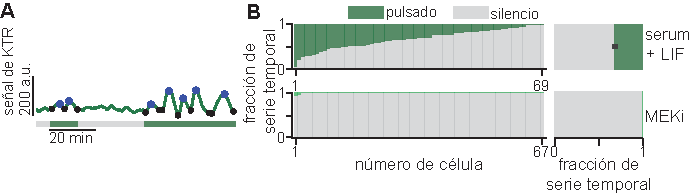
\includegraphics[width=1\textwidth]{figures/chapter2/C2_activity.pdf} 
    \caption{\textbf{La dinámica de pulsado es heterogénea.} (A) Actividad o proporción de tiempo de pulsado (barra verde inferior), y no pulsado o silencio (barra gris inferior) en una porción de una serie temporal de célula individual suavizada de la señal KTR en la condición de s+L (serie temporal superior). Los pulsos se indican por los máximos (puntos azules) y los mínimos correspondientes (puntos negros) que los definen. (B) Izquierda: fracción de tiempo que las células individuales pasaron pulsando (verde) o sin pulsar (gris) en serum + LIF solo (arriba) o al añadir MEKi (abajo). A la derecha: Tiempo medio que las células estuvieron pulsando (verde) o no pulsando (gris) en la población celular. La barra de error indica el el SEM (por \textit{standard error of the mean}).}
    \label{C2_fig:actividad}
\end{figure}


 \subsection{Medidas cuantitativas de pares de pulsos sucesivos}

Retomando ideas anteriores, las herramientas estándar de análisis de oscilaciones nos sugirieron signos oscilatorios no estacionarios en la dinámica de actividad de ERK (sección \ref{C2_sec:oscilaciones}). No obstante, fueron insuficientes para describir en simultáneo la presencia de pulsos aislados, que, producto de la inspección visual de las trazas, consideramos importante incorporar a nuestra descripción. Que los pulsos sean aislados o formen parte de intervalos oscilatorios está asociado a entender cómo están organizados los pulsos de actividad en las series temporales. Para esto, introdujimos un conjunto de medidas cuantitativas, cuya definición y análisis introduciremos a continuación.


En adelante, vamos a decir que  un pulso es sucesivo al otro cuando es el próximo pulso en la misma serie temporal. Para cuantificar el tiempo que transcurría entre un pulso y su siguiente, definimos el \textbf{intervalo de interpulsado} (IPI) $IPI_{i,j}$ entre un par de pulsos sucesivos $P_i, P_j$ con índices $j >i$ como el intervalo de tiempo entre sus máximos (figura \ref{C2_fig:analisis_pulsos_sucesivos}A)  \marginpar{intervalo de\\interpulsado}

\begin{equation}
    IPI_{i,j} = j-i.
    \label{C2_eq:IPI}
\end{equation}

 \begin{figure}
    \centering
    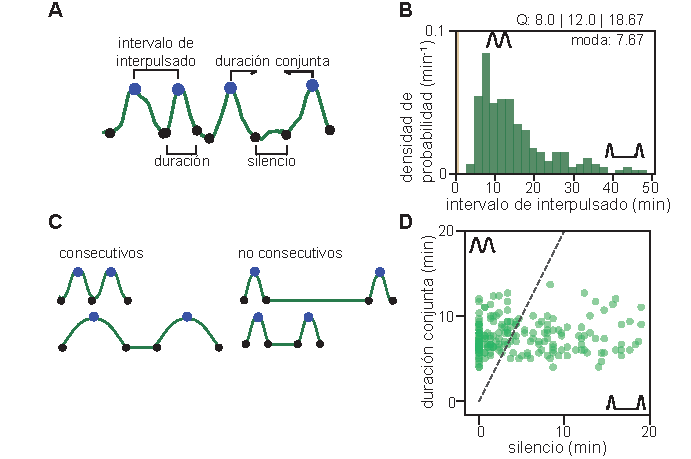
\includegraphics[width=1\columnwidth]{figures/chapter2/C2_IPI_consec.pdf}\caption{\textbf{Caracterización cuantitativa de pulsos sucesivos.} (A) Medidas cuantitativas de pulsos sucesivos indicadas en una porción de una traza de célula individual suavizada de la señal KTR en la condición de s+L. Los pulsos se indican por los máximos (puntos azules) y los mínimos correspondientes (puntos negros) que los definen. Por completitud, también se indica la duración de un pulso individual. (B) Distribución del intervalo de interpulsado para la condición serum + LIF. Se indica el límite de resolución del reconocimiento de pulsos (barra amarilla) y los cuartiles (Q) 25, 50 y 75. (C) Esquema de la definición de pares de pulsos consecutivos (arriba) y no consecutivos (abajo). (D) Duración conjunta un par de pulsos sucesivos en función del intervalo de silencio entre ellos (puntos verdes) en la condición de s+L. La línea discontinua con pendiente 2 clasifica los pares de pulsos consecutivos (arriba) y no consecutivos (abajo). El rango de los ejes se ajustó para resolver mejor los puntos de datos individuales, dejando fuera de la escala 27 de los 225 puntos de datos. Datos en (B,D) de N = 69 células y n = 225 pares de pulsos. }
    \label{C2_fig:analisis_pulsos_sucesivos}
\end{figure}


Los valores que puede tomar el IPI están limitados por la resolución impuesta por el algoritmo de reconocimiento de pulsos. Fijamos previamente la distancia mínima $|i-j|$ entre dos máximos $x_i, x_j \in M$ en 2 cuadros. Así, la distancia entre máximos de pulsos $P_k, P_l \in P$ verifica $ |k-l| \geq 2$ cuadros, y en particular $IPI_{k,l} \geq 2$ cuadros para cualquier par de pulsos sucesivos $P_k,P_l \in P$ (región amarilla en la figura \ref{C2_fig:analisis_pulsos_sucesivos}B). La distribución de IPI es marcadamente asimétrica, con una moda de $7.67$ min., similar a la moda de la duración de pulsos (figura \ref{C2_fig:analisis_pulsos_sucesivos}B). Para que el IPI tenga un valor similar al de las duraciones de los pulsos vecinos, un pulso debe comenzar inmediatamente después del anterior. Por lo tanto, esta similitud de las modas sugiere la presencia de pulsos consecutivos, que ocurren inmediatamente uno tras otro. Por otro lado, la cola larga de la distribución de IPI sugiere la presencia de pulsos muy lejanos uno del otro, es decir, no consecutivos.


Quisimos determinar qué tan habituales eran los pulsos consecutivos, y no consecutivos o aislados. Una manera simple de determinar si dos pulsos sucesivos son consecutivos es medir el tiempo que transcurre entre el final del primero y el inicio del segundo. Sin embargo, notamos que pulsos pertenecientes al mismo tren de pulsos tenían duraciones similares en comparación con la población de pulsos, donde ésta era más variable. Por ejemplo, a simple vista los pulsos de la célula $40$ son más largos que los de la célula $56$ en la figura \ref{C2_fig:traces}. Con esta observación, consideramos más adecuado incorporar a la definición de pulsos consecutivos una medida que contemple no sólo el tiempo transcurrido entre dos pulsos sucesivos sino también sus duraciones, puesto que es de esperar que pulsos más largos puedan acomodar fluctuaciones de mayor duración entre el fin del primero y el inicio del segundo. Entonces, determinamos que dos pulsos son consecutivos si tienen mínimos compartidos o están separados por intervalos de silencio que son cortos en relación con duración promedio, como ejemplificamos en la figura  \ref{C2_fig:analisis_pulsos_sucesivos}C. Para implementar esta definición, introducimos dos medidas: la duración conjunta y el intervalo de silencio entre pulsos sucesivos (figura \ref{C2_fig:analisis_pulsos_sucesivos}A).


Definimos la \textbf{duración conjunta} del pulso $dt_{i,j}$ entre un par de pulsos sucesivos $P_i, P_j$ donde $P_i$ ocurre antes que $P_j$ y $j >i$, como la suma de la duración derecha o de bajada del primer pulso $P_i$ y la duración izquierda o de subida del segundo pulso $P_j$ (figura \ref{C2_fig:analisis_pulsos_sucesivos}A) \marginpar{duración conjunta}
\begin{equation}
    dt_{i,j} = dt_i^{\text{right}} + dt_j^{\text{left}}.
\end{equation}
Además, definimos el \textbf{intervalo de silencio} $dm_{i,j}$ entre un par de pulsos sucesivos $P_i, P_j$ con $j >i$ como el tiempo transcurrido entre el final del primer pulso $P_i$ -marcado con su mínimo derecho- y el inicio del pulso segundo pulso $P_j$-marcado con su mínimo izquierdo- (figura \ref{C2_fig:analisis_pulsos_sucesivos}A) \marginpar{intervalo de\\silencio}
\begin{equation}
    dm_{i,j} = k_j - l_i.
\end{equation}
La distancia mínima $|i-j|$ entre dos mínimos $x_i, x_j \in m$ es de 2 cuadros. En consecuencia, dado un pulso $P_j=(j, kj, lj) \in P$, la distancia entre los dos mínimos que define el pulso $dm_j= k_j-l_j$ satisface $dm_j \geq 2$ cuadros. 


Graficamos la duración conjunta en función del silencio entre dos pulsos sucesivos en la figura \ref{C2_fig:analisis_pulsos_sucesivos}D. Al estas cantidades ser magnitudes calculadas para pares de pulsos sucesivos, cada punto en esta figura representa un par de pulsos sucesivos de una serie temporal. Con nuestra idea de consecutividad (figura \ref{C2_fig:analisis_pulsos_sucesivos}C), los pares de pulsos sucesivos separados entre sí poblarían la región inferior derecha, mientras que los pares de pulsos consecutivos la parte superior izquierda. 


Definimos los \textbf{pares de pulsos consecutivos} como aquellos con un intervalo de silencio inferior a la mitad de la duración del pulso conjunto, es decir, los pulsos sucesivos $P_i, P_j$ con $j >i$ son consecutivos si
\marginpar{pares de pulsos consecutivos}
\begin{equation}
    dm_{i,j} < \frac{1}{2} dt_{i,j}.
\end{equation} 
Dado que cada intervalo de interpulsado puede descomponerse en un intervalo de silencio y una duración conjunta del pulso (figura \ref{C2_fig:analisis_pulsos_sucesivos}A)
\begin{equation}
    IPI_{i,j} = dm_{i,j} + dt_{i,j},
\end{equation}
esta definición restringe de manera selectiva los intervalos de interpulsado entre pulsos consecutivos a tiempos pequeños. La definición de pares de pulsos consecutivos está representada en la línea punteada de la figura \ref{C2_fig:analisis_pulsos_sucesivos}D, donde los pares de pulsos consecutivos están por sobre esta línea. Con este criterio, el $52\%$ de todos los pares de pulsos en las células que crecen en s+L se sitúan por encima del umbral y se clasifican como consecutivos. 


Que la mayoría de los pares de pulsos sucesivos sean consecutivos explica el valor modal de la distribución de IPI de la figura \ref{C2_fig:analisis_pulsos_sucesivos}B, y complementa a los signos oscilatorios no estacionarios observados en la sección \ref{C2_sec:oscilaciones}. Sin embargo, esta información no es suficiente para entender cuál es el origen de la cola de tiempos largos que observamos en la distribución de IPI ni la proporción de pares de pulsos no consecutivos de la región inferior a la línea punteada de la figura \ref{C2_fig:analisis_pulsos_sucesivos}D.


\section{Descripción conceptual de la dinámica de ERK}
\label{C2_sec:pulsado_estoctastico}

Como las distribuciones asimétricas y de cola larga de IPI son una de las principales características de modelos de pulsado estocásticos de Poisson, en esta sección evaluamos la posibilidad de que los pulsos de ERK sean de naturaleza estocástica. Comenzamos por comparar los datos experimentales con dos modelos simples de pulsado estocástico de Poisson y, luego, proponemos una estrategia para cuantificar la longitud de los intervalos oscilatorios. 


\subsection{Hipótesis de pulsado estocástico}
\subsubsection*{Pulsado estocástico de población homogénea}

Un proceso de Poisson consiste en una serie de eventos independientes entre sí y del tiempo que ocurren con una tasa $\lambda > 0$ y los tiempos de espera $T$ entre dos eventos sucesivos se distribuyen según (\cite{TimeSeries1972,Levine2013})
\begin{equation}
    P(T;\lambda) = \lambda e^{-\lambda T},
\end{equation}
donde la distribución de tiempos de espera está totalmente caracterizada por un único parámetro $\lambda$. Calculamos la distribución de tiempos entre pulsos, o silencios, en los datos experimentales (figura \ref{C2_fig:pulsos_estocasticos_homog}A). Observamos que la distribución tenía una cola de tiempos grandes, consistente con un comportamiento exponencial. Esta observación refuerza la idea de que dinámica de pulsado estocástico que sugería la forma de la distribución de IPI. 

Para evaluar esta hipótesis de pulsado estocástico, comparamos nuestros experimentos con datos obtenidos de un modelo donde los tiempos entre los pulsos, o silencios, están distribuidos de manera exponencial. En vistas de obtener series temporales sintéticas, ajustamos el logaritmo de la distribución experimental de silencios mediante la función lineal 
\begin{equation}
    f(T;\lambda) = \log{\lambda} - \lambda T,
    \label{C2_eq:ajuste_homogeneo}
\end{equation}
estimamos el valor de $\lambda$ \cite{Harris2020}. Con este parámetro, generamos una distribución discreta de tiempos de espera muestreando de una distribución exponencial de parámetro $\lambda$ tantos puntos como pulsos había en el experimento (figura \ref{C2_fig:pulsos_estocasticos_homog}B). Luego, esta fue la distribución de tiempos de espera a partir de la cual obtuvimos las series temporales sintéticas.  

A continuación, generamos tantas series temporales como células habíamos medido en el experimento. La duración de cada serie temporal sintética era equivalente a la de una traza experimental. Muestreamos el tiempo de espera hasta el comienzo de cada pulso a partir de la distribución exponencial de la figura \ref{C2_fig:pulsos_estocasticos_homog}B, la duración de cada pulso era una muestra aleatoria de la distribución experimental de la duración del pulso de la figura \ref{C2_fig:amp_durac}B y las series temporales siempre comenzaban con un intervalo de silencio. Representamos los pulsos como cuadrados y anotamos sus picos en el centro (figura \ref{C2_fig:pulsos_estocasticos_homog}C). Analizamos estas series temporales estocásticas siguiendo el mismo protocolo de análisis que utilizamos para los datos experimentales, detallado anteriormente. No incluimos en el análisis los pulsos que se extendieron más allá del final de la serie temporal. 


\begin{figure}
    \centering
    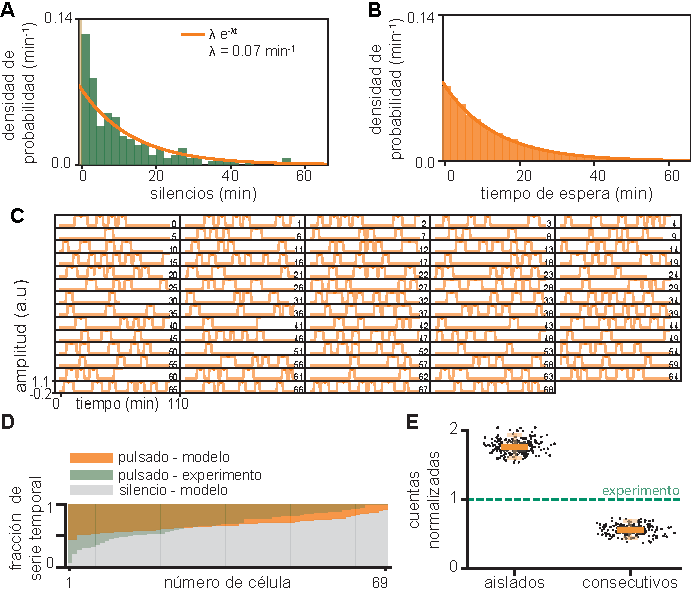
\includegraphics[width=1\columnwidth]{figures/chapter2/C2_pulsado_estocastico_homog.pdf}\caption{\textbf{Modelo estocástico de pulsado de población homogénea.}(A) Distribución de los intervalos de silencio (barras verdes) definidos como el tiempo entre dos pulsos sucesivos, para la condición de serum + LIF (n = 225 pares de pulsos). Ajuste exponencial utilizado en el modelo de población homogénea (línea naranja). (B) Distribución del tiempo de espera (barras naranjas) muestreada a partir del ajuste exponencial en A (línea naranja).(C) Series temporales generadas a partir del modelo de población homogénea (línea naranja), con los máximos de los pulsos (puntos). Las duraciones de los pulsos se eligieron al azar de la distribución experimental en la figura \ref{C2_fig:amp_durac}C. Las longitudes de las trazas corresponden a la longitud de las trazas experimentales mostradas en la figura \ref{C2_fig:traces}. (D) Fracción de tiempo que las series temporales individuales simuladas pasaron pulsando (naranja), en comparación con los datos experimentales (verde). (E) Recuentos de pulsos aislados y consecutivos de 200 realizaciones del modelo divididos por los recuentos correspondientes en las trazas experimentales (puntos negros). Una sola realización se compone N = 69 trazas. Las barras de color representan la mediana, los límites de la caja son los percentiles 25 y 75 de las distribuciones, y los bigotes son los percentiles 5 y 95. }
    \label{C2_fig:pulsos_estocasticos_homog}
\end{figure}


En la figura \ref{C2_fig:pulsos_estocasticos_homog}D podemos observar la fracción de tiempo que cada célula sintética pulsa. Si bien el modelo pudo reproducir los valores intermedios de actividad que medimos en el experimento, encontramos que las simulaciones no pudieron recapitular la presencia de células que pulsan durante una fracción de tiempo muy larga (izquierda en la figura \ref{C2_fig:pulsos_estocasticos_homog}D), así como las células que pulsan durante una fracción de tiempo muy corta que observamos en el experimento (derecha en la figura \ref{C2_fig:pulsos_estocasticos_homog}D). 


Para entender si los datos sintéticos podían recapitular cómo estaban ordenados los pulsos en las series temporales, comparamos la cantidad de pulsos consecutivos y aislados en los datos experimentales y en las simulaciones. Para esto, definimos la cantidad de \textbf{pulsos consecutivos} como el número de pulsos que eran parte de al menos un par de pulsos consecutivos, y la cantidad de \textbf{pulsos aislados} como el número de pulsos que no eran consecutivos.\marginpar{pulsos consecutivos\\y aislados} Observamos que los pulsos aislados en las simulaciones ocurrían con más frecuencia que en el experimento, mientras que los pulsos consecutivos ocurrían en una fracción menor (figura \ref{C2_fig:pulsos_estocasticos_homog}E). Esta comparación nos indicó que un modelo de pulsado estocástico en donde la distribución de tiempos de espera está regulada por un solo parámetro no es suficiente para reproducir los datos experimentales. 


Previamente, observamos actividad heterogénea en los datos experimentales. Por otro lado, en nuestra descripción establecimos que una sola tasa $\lambda$ regulaba la dinámica de tiempo entre pulsos. Ajustando un solo parámetro a todas las series temporales experimentales en la ecuación \ref{C2_eq:ajuste_homogeneo}, indirectamente asumimos que esta heterogeneidad era consecuencia de la descripción de la actividad dinámica de ERK y de la duración de las mediciones. Con esta descripción no fue posible reproducir la distribución de actividad experimental, pero el modelo sí fue capaz de reproducir los valores intermedios de actividad que medimos en el experimento. Este resultado nos motiva a explorar la idea de que esta heterogeneidad que observamos en los experimentos no sea consecuencia de la descripción de la actividad dinámica de ERK, sino que tenga origen en una heterogeneidad propia celular. Esta heterogeneidad propia celular podría estar dada por diferencias estables entre las células, o diferencias que surjan de efectos con escalas temporales grandes comparadas con nuestras mediciones de aproximadamente 2 horas. 


\subsubsection*{Pulsado estocástico de población heterogénea}

A continuación, comparamos los datos experimentales con una hipótesis que contemplara una variabilidad celular. La hipótesis detrás de esta idea es la de establecer un parámetro $\lambda_i$ para cada célula $i$, y los tiempos de espera en cada caso estén gobernados por una distribución exponencial de la ecuación \ref{C2_eq:ajuste_homogeneo} propia de cada célula. Sin embargo, ajustar un parámetro  $\lambda_i$ para cada traza $i$ no era posible dada la baja cantidad de pulsos en cada serie temporal. Dada esta limitación, decidimos tomar un enfoque distinto para evaluar esta nueva hipótesis. Dada una serie temporal experimental con $n_i$ pulsos y duración $L_i$, buscamos obtener una serie temporal sintética análoga de duración $T_i$. En este caso, buscamos mezclar en el tiempo la ubicación de los $n_i$ pulsos al azar, de manera de conservar la cantidad de pulsos por unidad de tiempo de en cada serie temporal. 


Para cada serie temporal sintética $i$, determinamos una sola duración de pulsos $dt_i$ como el promedio de la duración de los pulsos de la traza experimental asociada $i$ y una duración $L_i$. Luego, colocamos el primer pulso en una posición aleatoria de la traza vacía. El intervalo de tiempo ocupado por este pulso era $dt_i$. Repetimos el procedimiento con el segundo pulso. Si el pulso comenzaba o terminaba dentro del primer pulso, o si el pulso terminaba después del final de la serie temporal, considerábamos que se trataba de una iteración fallida. Intentamos de nuevo colocar hasta tener éxito, o hasta realizar $10^{7}$ iteraciones fallidas. Repetimos este procedimiento hasta colocar (idealmente) $n_i$ pulsos en la serie temporal sintética. De esta manera, el número de pulsos en cada traza sintética estaba limitado por el número total de pulsos en la traza experimental. Representamos los pulsos como cuadrados y anotamos sus picos en el centro (figura \ref{C2_fig:pulsos_estocasticos_heterog}B). Analizamos estas series temporales sintéticas siguiendo el mismo protocolo de análisis que utilizamos para los datos experimentales. 



 \begin{figure}
    \centering
    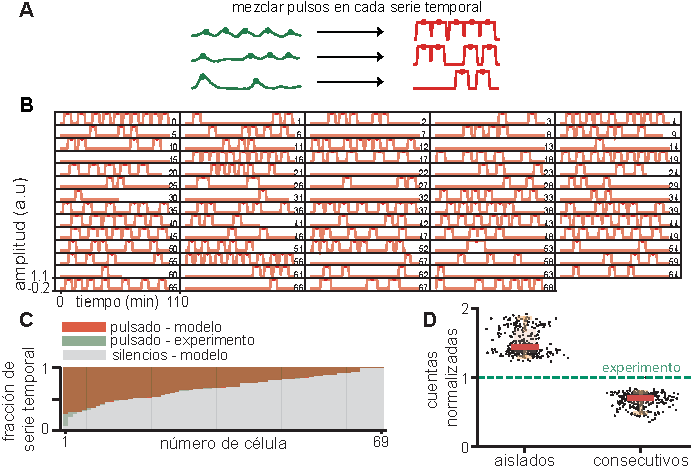
\includegraphics[width=1\columnwidth]{figures/chapter2/C2_pulsado_estocastico_heterog.pdf}\caption{\textbf{Modelo estocástico de pulsado de población heterogénea.}(A) Esquema del modelo de pulsación estocástica de población heterogénea. Los pulsos en las trazas experimentales individuales (izquierda, verde) se reposicionaron para generar trazas con pulsos mezclados al azar en el tiempo (derecha, rojo). (B) Series temporales generadas a partir del modelo de población heterogénea (línea roja), con los máximos de pulso (puntos). Todas las duraciones de los pulsos en una serie temporal se establecieron como la duración media del pulso en la traza experimental correspondiente. Las longitudes de las trazas corresponden a la longitud de las trazas experimentales mostradas en la figura \ref{C2_fig:traces}. (C) Fracción de tiempo que las células pasaron pulsando (rojo). (D) Recuentos normalizados de pulsos aislados y consecutivos de 200 realizaciones del modelo, cada una de las cuales consta de N = 69 trazas mezcladas. Las barras de color representan la mediana, los límites de la caja son los percentiles 25 y 75 de las distribuciones, y los bigotes son los percentiles 5 y 95. }
    \label{C2_fig:pulsos_estocasticos_heterog}
\end{figure}


Con este modelo esperábamos describir correctamente el análisis de actividad de la figura \ref{C2_fig:actividad}, pues mezclar pulsos de una serie temporal no debería alterar esta medida. En la figura \ref{C2_fig:pulsos_estocasticos_heterog}C podemos observar que la fracción de tiempo que cada célula sintética pulsa reproduce correctamente los datos experimentales. En la figura  \ref{C2_fig:pulsos_estocasticos_heterog}D comparamos la cantidad de pulsos consecutivos y aislados en las simulaciones con los datos experimentales. Podemos ver que el modelo de pulsación estocástica de población heterogénea sobrestima la cantidad de pulsos aislados, y subestima la cantidad de pulsos consecutivos de los experimentos, siendo incapaz de reproducir este aspecto de la dinámica de actividad de ERK en ESCs. Este resultado sugiere que los pulsos de actividad de ERK tienen un orden determinado, y no es posible reproducir ese orden mezclando los pulsos al azar.



Como conclusión, observamos que los modelos de pulsación estocástica simples no pueden reproducir la forma en la que los pulsos están ordenados en las series temporales experimentales: sobrestiman los pulsos aislados y subestiman los pulsos consecutivos. Este resultado nos informa que la dinámica de activación de ERK no es una pulsación estocástica, y que la manera en que los pulsos están ordenados es una característica distintiva de esta dinámica. Que la proporción de pulsos consecutivos sea la principal diferencia que encontramos entre los modelos de pulsado estocástico y los datos nos conduce a analizar con mayor profundidad el orden de los pulsos consecutivos. 


\subsection{Secuencias de pulsos consecutivos}
\label{C2_ssec:seq_pulsos_cons}


Buscamos analizar con qué frecuencia se producían en las series temporales experimentales en \textbf{secuencias o trenes de un determinado número de pulsos consecutivos}\marginpar{secuencias de pulsos consecutivos}. Para este fin, retomamos clasificación de pares de pulsos consecutivos y no consecutivos de la figura \ref{C2_fig:analisis_pulsos_sucesivos}D. Ordenamos los pares de pulsos sucesivos de cada serie temporal $i$ en vectores $V^i_2$ según el tiempo en el que aparecían en la traza. Cada vector $i$ tenía una dimensión equivalente al total de pares sucesivos de pulsos de la serie temporal $i$, y cada coordenada, que correspondía a un par de pulsos sucesivos, le asignamos una etiqueta. La etiqueta era $1$ si el par de pulsos había sido clasificado como consecutivo, y $0$ en caso contrario. Con esta estrategia, el número de trenes de pulsos de $2$ pulsos era la suma de las componentes del vector (figura \ref{C2_fig:seq_pulsos_consecutivos}A).


Para calcular el número de trenes con $3$ pulsos consecutivos, por cada vector $V^i_2$ generamos un nuevo vector $V^i_3$ definido como el producto de las etiquetas adyacentes de $V^i_2$. En $V^i_3$, cada entrada representaba grupos de tres pulsos sucesivos, y tenía un valor de 1 si el primer y el segundo pulso, y el segundo y el tercero fueron previamente clasificados como consecutivos, y 0 en caso contrario (figura \ref{C2_fig:seq_pulsos_consecutivos}A). Obtuvimos el número de trenes con 3 pulsos consecutivos como la suma de todas las etiquetas de $V^i_3$. Para determinar el número de trenes con 4, 5, 6, ... pulsos consecutivos, iteramos este procedimiento: primero generamos una lista multiplicando las etiquetas adyacentes de la lista anterior, y luego sumamos las etiquetas de la lista resultante (figura \ref{C2_fig:seq_pulsos_consecutivos}A).


 \begin{figure}
    \centering
    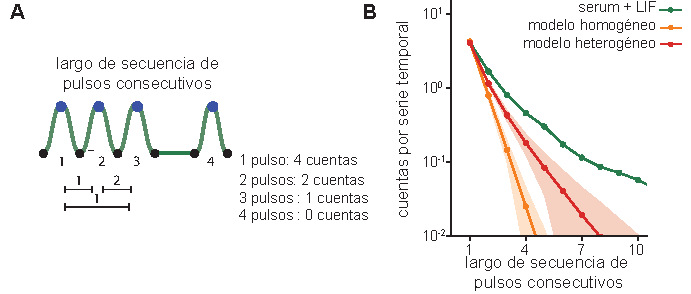
\includegraphics[width=1\columnwidth]{figures/chapter2/C2_seq_pulsos_consecutivos.pdf}\caption{\textbf{Análisis de trenes de pulsos consecutivos muestra una característica distintiva de los datos experimentales}. (A) Esquema del criterio de conteo del largo de secuencias de trenes de pulsos consecutivos. (B) Número de trenes de pulsos en función del número de pulsos consecutivos en el tren para los datos experimentales (verde), modelo de población homogénea (naranja) y modelo de población heterogénea (rojo). Normalizamos los recuentos por el número de series temporales de cada grupo de datos. El área sombreada es desviación estándar de 200 realizaciones independientes de los modelos estocásticos.}
    \label{C2_fig:seq_pulsos_consecutivos} %El primer punto de datos corresponde al número total de pulsos individuales.
\end{figure}


En la figura \ref{C2_fig:seq_pulsos_consecutivos}B se encuentran las mediciones del número de trenes de pulsos consecutivos de determinada duración realizadas sobre los datos experimentales y las series sintéticas de los modelos de pulsado estocástico. El primer punto de este gráfico corresponde al número total de pulsos individuales, en donde los experimentos parecen coincidir con las simulaciones. Sin embargo, observamos que el experimento presenta sistemáticamente mayor frecuencia de trenes de pulsos consecutivos que los modelos de pulsado estocástico. 


En resumen, la frecuencia de secuencias de pulsos consecutivos de determinada duración que logramos medir en los datos experimentales cuantifica una característica distintiva de los datos experimentales. Que los modelos de pulsados estocásticos simples que consideramos fallen en reproducir esta característica complementa las observaciones de signos oscilatorios no estacionarios que muestran las herramientas de análisis estándar de oscilaciones que implementamos en la sección \ref{C2_sec:oscilaciones}. Con esta idea, creemos que la cantidad de trenes de pulsos consecutivos de determinada duración es una característica primordial que cualquier descripción teórica que pretenda describir los datos debe ser capaz de reproducir.


\section{Conclusiones y discusión}

Con el objetivo de estudiar cómo es la dinámica de activación de ERK en células madre embrionarias de ratón en condiciones de cultivo que mantienen la pluripotencia, en este capítulo presentamos la primera caracterización cuantitativa de la dinámica de activación de ERK en células madre embrionarias, donde nos enfocamos en escalas temporales cortas. Nuestro sistema de estudio fueron células madre embrionarias de ratón \textit{wild type} crecidas en serum + LIF, condiciones de cultivo que mantienen la pluripotencia y simultáneamente activan ERK. 


Primero realizamos mediciones con un sensor de traslocación para obtener series temporales que representaban la dinámica de activación de ERK en células individuales (figuras \ref{C2_fig:FRET}, \ref{C2_fig:KTR}, \ref{C2_fig:traces}). A partir de estas mediciones observamos que la actividad de ERK era pulsátil en ESCs. Esta actividad pulsátil presentó una amplia gama de comportamientos dinámicos: algunas células mostraron actividad pulsátil regular, otras mostraron solamente pulsos aislados, y también observamos células con transiciones entre intervalos de pulsado regulares, intervalos de silencio y pulsos aislados. 


Para responder a la pregunta de si los intervalos de pulsado regular eran oscilatorios, estudiamos los signos oscilatorios globales de las series temporales experimentales individuales a partir de analizar su espectro de potencias y su función de autocorrelación (figura \ref{C2_fig:FFT_AC}). Encontramos que estas herramientas de análisis de oscilaciones sugerían un comportamiento oscilatorio en una porción de los datos de s+L. Sin embargo, la heterogeneidad que observamos en estos análisis respaldaba la idea de que la actividad de ERK viene en un abanico de comportamientos dinámicos distintos, y estas herramientas fueron insuficientes para describirlos. Implementando la transformada \textit{Wavelet}, observamos que el espectro de potencias local de las series temporales experimentales sugería signos oscilatorios no estacionarios en la condición donde ERK estaba activa, resultado que reforzaba nuestras observaciones (figuras \ref{C2_fig:wavelets_MEKI},\ref{C2_fig:wavelets_WT}). Sin embargo, estas estrategias de análisis no lograron capturar los principales aspectos dinámicos 
 que observábamos de manera satisfactoria. 
 

Como alternativa, desarrollamos un protocolo para detectar pulsos de actividad en las series temporales como las que adquirimos experimentalmente (figura \ref{C2_fig:algoritmo_pulse_detection}). Calibramos este método considerando que las fluctuaciones de base dominaban las mediciones realizadas sobre del control negativo, y que el algoritmo debería maximizar la cantidad de pulsos detectados en la condición s+L (figura \ref{C2_fig:umbrales}). El resultado de este algoritmo de detección fueron máximos que marcaban los picos de cada pulso, con dos mínimos locales asociados que marcaban el comienzo y el final de cada pulso. Obtener un resultado de estas características nos permitió realizar la caracterización cuantitativa de la dinámica de activación de ERK, que realizamos a partir de definir varios observables que resumían las principales propiedades de la dinámica pulsátil de las series temporales. 


Observamos que la fracción total de tiempo que las células individuales pulsaban era variable (\ref{C2_fig:actividad}). Se cree que la forma en que las células de la masa celular interna se especifican hacia el endodermo primitivo y el epiblasto para dar lugar al patrón de sal y pimienta (capítulo \ref{ch1}) podría depender distintas fuentes de heterogeneidad celular como la actividad variable de las vías de señalización involucradas en ese momento del desarrollo \cite{Pokrass2020,Saiz2016}. En este contexto, la heterogeneidad que observamos en la dinámica de activación de ERK en ESCs podría ser relevante para profundizar en la comprensión sobre decisiones del destino celular en las células pluripotentes. Sin embargo, la duración de nuestras mediciones nos impiden distinguir si esta variabilidad resulta de diferencias estables en el comportamiento dinámico entre las células, o de que las células individuales tengan transiciones entre estados oscilatorios activos e inactivos en escalas temporales largas en comparación con las mediciones. Con esta motivación, en el capítulo \ref{ch4} exploramos estas alternativas. 


Observamos que la distribución de intervalos de interpulsado era marcadamente asimétrica (figura \ref{C2_fig:analisis_pulsos_sucesivos}). Por un lado, la moda de la distribución de intervalo de interpulsado era similar a la de la duración de pulsos (figura \ref{C2_fig:amp_durac}), sugiriendo la presencia de pulsos consecutivos. Reforzamos esta observación determinando la cantidad de pares de pulsos consecutivos en las trazas experimentales, donde impusimos que dos pulsos eran consecutivos si tenían mínimos compartidos o separados por intervalos de silencio cortos en relación con duración promedio. Nuestro análisis indicó que la mayoría de los pares de pulsos sucesivos eran consecutivos (figura \ref{C2_fig:analisis_pulsos_sucesivos}).


Por otro lado, la cola de tiempos largos de la distribución de IPI era consistente con modelos de pulsado estocásticos de Poisson, comportamientos que fueron observados previamente en células más diferenciadas (capítulo \ref{ch1}). Sin embargo, los modelos de pulsados estocásticos simples no lograron reproducir la forma en la que los pulsos están ordenados en las series temporales experimentales: sobrestimaron la proporción de los pulsos aislados y subestimaron la de los pulsos consecutivos (figuras \ref{C2_fig:pulsos_estocasticos_homog}, \ref{C2_fig:pulsos_estocasticos_heterog}). En esta línea, observamos que, en los experimentos, la frecuencia de trenes de pulsos de determinada duración eran inconsistentes con los modelos de pulsados estocásticos (figura \ref{C2_fig:seq_pulsos_consecutivos}), característica que consideramos que debe reproducir cualquier descripción teórica que pretenda describir los experimentos.
En otros tipos celulares más diferenciados se ha descripto que la dinámica de activación de ERK es en forma de pulsado estocástico. En las ESCs, los modelos de pulsos estocásticos simples no lograron capturar las estadísticas de los pulsos aislados y consecutivos observados en los experimentos, lo que sugiere que este tipo de descripciones dinámicas no aplican a ESCs. 


Que los modelos de pulsados estocásticos simples que consideramos fallaran en reproducir esta característica complementa las observaciones de signos oscilatorios no estacionarios que mostraron las herramientas de análisis estándar de oscilaciones y el hecho de que los pares de pulsos sucesivos sean mayoritariamente consecutivos. Como complemento, inferimos que la cola de tiempos largos que observamos en la distribución de IPI es reflejo de la presencia de pulsos aislados o trenes de pulsos separados por intervalos de silencios en las series temporales de ERK. 


En definitiva, interpretamos a partir de nuestro análisis que los pulsos de ERK en ESCs que crecen en condiciones de cultivo que mantienen la pluripotencia tienen una duración característica y, a menudo forman parte de intervalos oscilatorios, intercalados con intervalos de silencios y pulsos aislados. Esta dinámica previamente no descripta la llamamos oscilaciones intermitentes. 


Esta caracterización de la dinámica de activación de ERK en células madre embrionarias fue posible gracias a la combinación del sensor de traslocación con filmaciones de alta resolución temporal. Como mencionamos en el capítulo \ref{ch1}, previamente se examinó la dinámica de ERK tras la estimulación aguda, estudio que se centró en la actividad de ERK en escalas temporales lentas y no resolvió las oscilaciones intermitentes de escalas temporales cortas que nosotros informamos \cite{Deathridge2019}. En particular, esta dinámica previamente no detectada, tiene un IPI modal de aproximadamente 7 minutos (es decir, unos 8 pulsos/h), y son por tanto mucho más rápidos que en cualquier otro sistema celular descrito hasta ahora. Sin embargo, a partir de nuestras mediciones no fue posible determinar caracterizar la amplitud de la dinámica de activación de ERK. Esta caracterización puede ser posible conociendo la relación funcional entre la amplitud de la señal del sensor KTR y la activación de ERK a través de, por ejemplo, modelar el funcionamiento del sensor KTR que utilizamos.


Por último, en los sistemas celulares que muestran pulsación estocástica de ERK, el aumento de los niveles de ligando conduce a IPIs más cortos y, por lo tanto, a un aumento de la tasa de pulsado \cite{Albeck2013}. Esto se ha interpretado como una codificación de la concentración de ligando a través de la modulación de la frecuencia \cite{Li2019}. En las ESCs, la frecuencia de pulsado podría transmitir información sobre los niveles de ligando, y en el próximo capítulo exploramos esta hipótesis.  
 
\end{document}




